% Created by tikzDevice version 0.12 on 2019-05-09 12:18:03
% !TEX encoding = UTF-8 Unicode
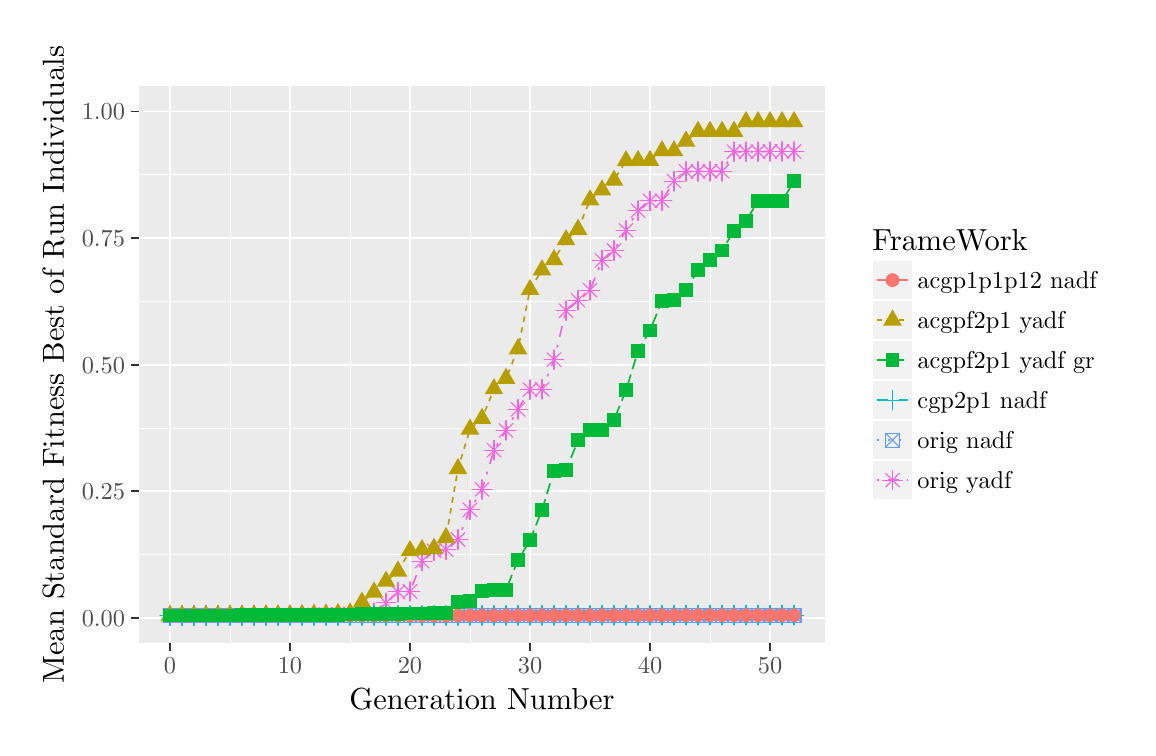
\begin{tikzpicture}[x=1pt,y=1pt]
\definecolor{fillColor}{RGB}{255,255,255}
\path[use as bounding box,fill=fillColor,fill opacity=0.00] (0,0) rectangle (397.48,252.94);
\begin{scope}
\path[clip] (  0.00,  0.00) rectangle (397.48,252.94);
\definecolor{drawColor}{RGB}{255,255,255}
\definecolor{fillColor}{RGB}{255,255,255}

\path[draw=drawColor,line width= 0.6pt,line join=round,line cap=round,fill=fillColor] (  0.00,  0.00) rectangle (397.48,252.95);
\end{scope}
\begin{scope}
\path[clip] ( 40.14, 30.56) rectangle (288.20,231.75);
\definecolor{fillColor}{gray}{0.92}

\path[fill=fillColor] ( 40.14, 30.56) rectangle (288.20,231.75);
\definecolor{drawColor}{RGB}{255,255,255}

\path[draw=drawColor,line width= 0.3pt,line join=round] ( 40.14, 62.57) --
	(288.20, 62.57);

\path[draw=drawColor,line width= 0.3pt,line join=round] ( 40.14,108.29) --
	(288.20,108.29);

\path[draw=drawColor,line width= 0.3pt,line join=round] ( 40.14,154.02) --
	(288.20,154.02);

\path[draw=drawColor,line width= 0.3pt,line join=round] ( 40.14,199.75) --
	(288.20,199.75);

\path[draw=drawColor,line width= 0.3pt,line join=round] ( 73.10, 30.56) --
	( 73.10,231.75);

\path[draw=drawColor,line width= 0.3pt,line join=round] (116.47, 30.56) --
	(116.47,231.75);

\path[draw=drawColor,line width= 0.3pt,line join=round] (159.83, 30.56) --
	(159.83,231.75);

\path[draw=drawColor,line width= 0.3pt,line join=round] (203.20, 30.56) --
	(203.20,231.75);

\path[draw=drawColor,line width= 0.3pt,line join=round] (246.57, 30.56) --
	(246.57,231.75);

\path[draw=drawColor,line width= 0.6pt,line join=round] ( 40.14, 39.70) --
	(288.20, 39.70);

\path[draw=drawColor,line width= 0.6pt,line join=round] ( 40.14, 85.43) --
	(288.20, 85.43);

\path[draw=drawColor,line width= 0.6pt,line join=round] ( 40.14,131.16) --
	(288.20,131.16);

\path[draw=drawColor,line width= 0.6pt,line join=round] ( 40.14,176.88) --
	(288.20,176.88);

\path[draw=drawColor,line width= 0.6pt,line join=round] ( 40.14,222.61) --
	(288.20,222.61);

\path[draw=drawColor,line width= 0.6pt,line join=round] ( 51.41, 30.56) --
	( 51.41,231.75);

\path[draw=drawColor,line width= 0.6pt,line join=round] ( 94.78, 30.56) --
	( 94.78,231.75);

\path[draw=drawColor,line width= 0.6pt,line join=round] (138.15, 30.56) --
	(138.15,231.75);

\path[draw=drawColor,line width= 0.6pt,line join=round] (181.52, 30.56) --
	(181.52,231.75);

\path[draw=drawColor,line width= 0.6pt,line join=round] (224.88, 30.56) --
	(224.88,231.75);

\path[draw=drawColor,line width= 0.6pt,line join=round] (268.25, 30.56) --
	(268.25,231.75);
\definecolor{drawColor}{RGB}{248,118,109}

\path[draw=drawColor,line width= 0.6pt,line join=round] ( 51.41, 40.49) --
	( 55.75, 40.51) --
	( 60.09, 40.51) --
	( 64.42, 40.51) --
	( 68.76, 40.51) --
	( 73.10, 40.51) --
	( 77.43, 40.51) --
	( 81.77, 40.51) --
	( 86.11, 40.51) --
	( 90.44, 40.51) --
	( 94.78, 40.51) --
	( 99.12, 40.51) --
	(103.45, 40.51) --
	(107.79, 40.51) --
	(112.13, 40.52) --
	(116.47, 40.52) --
	(120.80, 40.52) --
	(125.14, 40.52) --
	(129.48, 40.52) --
	(133.81, 40.53) --
	(138.15, 40.53) --
	(142.49, 40.53) --
	(146.82, 40.53) --
	(151.16, 40.54) --
	(155.50, 40.54) --
	(159.83, 40.54) --
	(164.17, 40.54) --
	(168.51, 40.55) --
	(172.84, 40.55) --
	(177.18, 40.55) --
	(181.52, 40.56) --
	(185.85, 40.56) --
	(190.19, 40.57) --
	(194.53, 40.57) --
	(198.86, 40.57) --
	(203.20, 40.58) --
	(207.54, 40.59) --
	(211.87, 40.59) --
	(216.21, 40.59) --
	(220.55, 40.60) --
	(224.88, 40.60) --
	(229.22, 40.60) --
	(233.56, 40.60) --
	(237.89, 40.60) --
	(242.23, 40.61) --
	(246.57, 40.61) --
	(250.90, 40.61) --
	(255.24, 40.62) --
	(259.58, 40.62) --
	(263.91, 40.62) --
	(268.25, 40.62) --
	(272.59, 40.62) --
	(276.92, 40.63);
\definecolor{drawColor}{RGB}{183,159,0}

\path[draw=drawColor,line width= 0.6pt,dash pattern=on 2pt off 2pt ,line join=round] ( 51.41, 40.51) --
	( 55.75, 40.53) --
	( 60.09, 40.53) --
	( 64.42, 40.55) --
	( 68.76, 40.57) --
	( 73.10, 40.58) --
	( 77.43, 40.61) --
	( 81.77, 40.65) --
	( 86.11, 40.69) --
	( 90.44, 40.72) --
	( 94.78, 40.76) --
	( 99.12, 40.86) --
	(103.45, 40.95) --
	(107.79, 41.02) --
	(112.13, 41.22) --
	(116.47, 41.40) --
	(120.80, 45.32) --
	(125.14, 48.96) --
	(129.48, 52.89) --
	(133.81, 56.55) --
	(138.15, 63.91) --
	(142.49, 64.31) --
	(146.82, 64.78) --
	(151.16, 68.66) --
	(155.50, 93.58) --
	(159.83,107.85) --
	(164.17,111.72) --
	(168.51,122.42) --
	(172.84,126.20) --
	(177.18,136.86) --
	(181.52,158.29) --
	(185.85,165.42) --
	(190.19,169.09) --
	(194.53,176.29) --
	(198.86,180.04) --
	(203.20,190.67) --
	(207.54,194.26) --
	(211.87,197.80) --
	(216.21,204.83) --
	(220.55,204.90) --
	(224.88,204.90) --
	(229.22,208.42) --
	(233.56,208.42) --
	(237.89,211.94) --
	(242.23,215.45) --
	(246.57,215.45) --
	(250.90,215.45) --
	(255.24,215.45) --
	(259.58,218.97) --
	(263.91,218.97) --
	(268.25,218.97) --
	(272.59,218.97) --
	(276.92,218.97);
\definecolor{drawColor}{RGB}{0,186,56}

\path[draw=drawColor,line width= 0.6pt,dash pattern=on 4pt off 2pt ,line join=round] ( 51.41, 40.50) --
	( 55.75, 40.51) --
	( 60.09, 40.52) --
	( 64.42, 40.52) --
	( 68.76, 40.53) --
	( 73.10, 40.54) --
	( 77.43, 40.57) --
	( 81.77, 40.59) --
	( 86.11, 40.60) --
	( 90.44, 40.62) --
	( 94.78, 40.65) --
	( 99.12, 40.69) --
	(103.45, 40.73) --
	(107.79, 40.75) --
	(112.13, 40.79) --
	(116.47, 40.90) --
	(120.80, 40.95) --
	(125.14, 40.99) --
	(129.48, 41.03) --
	(133.81, 41.12) --
	(138.15, 41.24) --
	(142.49, 41.29) --
	(146.82, 41.36) --
	(151.16, 41.57) --
	(155.50, 45.42) --
	(159.83, 45.64) --
	(164.17, 49.30) --
	(168.51, 49.79) --
	(172.84, 49.87) --
	(177.18, 60.55) --
	(181.52, 67.71) --
	(185.85, 78.65) --
	(190.19, 92.87) --
	(194.53, 93.00) --
	(198.86,103.80) --
	(203.20,107.51) --
	(207.54,107.51) --
	(211.87,111.26) --
	(216.21,121.90) --
	(220.55,136.16) --
	(224.88,143.52) --
	(229.22,154.26) --
	(233.56,154.42) --
	(237.89,158.21) --
	(242.23,165.28) --
	(246.57,168.89) --
	(250.90,172.42) --
	(255.24,179.57) --
	(259.58,183.19) --
	(263.91,190.22) --
	(268.25,190.29) --
	(272.59,190.29) --
	(276.92,197.42);
\definecolor{drawColor}{RGB}{0,191,196}

\path[draw=drawColor,line width= 0.6pt,dash pattern=on 4pt off 4pt ,line join=round] ( 51.41, 40.51) --
	( 55.75, 40.51) --
	( 60.09, 40.51) --
	( 64.42, 40.51) --
	( 68.76, 40.51) --
	( 73.10, 40.51) --
	( 77.43, 40.51) --
	( 81.77, 40.52) --
	( 86.11, 40.52) --
	( 90.44, 40.52) --
	( 94.78, 40.52) --
	( 99.12, 40.52) --
	(103.45, 40.52) --
	(107.79, 40.52) --
	(112.13, 40.52) --
	(116.47, 40.52) --
	(120.80, 40.53) --
	(125.14, 40.53) --
	(129.48, 40.53) --
	(133.81, 40.53) --
	(138.15, 40.53) --
	(142.49, 40.53) --
	(146.82, 40.54) --
	(151.16, 40.54) --
	(155.50, 40.54) --
	(159.83, 40.55) --
	(164.17, 40.55) --
	(168.51, 40.56) --
	(172.84, 40.56) --
	(177.18, 40.57) --
	(181.52, 40.57) --
	(185.85, 40.58) --
	(190.19, 40.58) --
	(194.53, 40.58) --
	(198.86, 40.59) --
	(203.20, 40.59) --
	(207.54, 40.61) --
	(211.87, 40.61) --
	(216.21, 40.61) --
	(220.55, 40.62) --
	(224.88, 40.64) --
	(229.22, 40.64) --
	(233.56, 40.65) --
	(237.89, 40.65) --
	(242.23, 40.66) --
	(246.57, 40.66) --
	(250.90, 40.66) --
	(255.24, 40.66) --
	(259.58, 40.66) --
	(263.91, 40.66) --
	(268.25, 40.67) --
	(272.59, 40.67) --
	(276.92, 40.68);
\definecolor{drawColor}{RGB}{97,156,255}

\path[draw=drawColor,line width= 0.6pt,dash pattern=on 1pt off 3pt ,line join=round] ( 51.41, 40.50) --
	( 55.75, 40.50) --
	( 60.09, 40.51) --
	( 64.42, 40.51) --
	( 68.76, 40.51) --
	( 73.10, 40.51) --
	( 77.43, 40.51) --
	( 81.77, 40.51) --
	( 86.11, 40.51) --
	( 90.44, 40.51) --
	( 94.78, 40.51) --
	( 99.12, 40.51) --
	(103.45, 40.51) --
	(107.79, 40.52) --
	(112.13, 40.52) --
	(116.47, 40.52) --
	(120.80, 40.52) --
	(125.14, 40.52) --
	(129.48, 40.52) --
	(133.81, 40.53) --
	(138.15, 40.53) --
	(142.49, 40.53) --
	(146.82, 40.53) --
	(151.16, 40.53) --
	(155.50, 40.53) --
	(159.83, 40.53) --
	(164.17, 40.54) --
	(168.51, 40.54) --
	(172.84, 40.54) --
	(177.18, 40.55) --
	(181.52, 40.55) --
	(185.85, 40.55) --
	(190.19, 40.55) --
	(194.53, 40.55) --
	(198.86, 40.56) --
	(203.20, 40.56) --
	(207.54, 40.56) --
	(211.87, 40.56) --
	(216.21, 40.56) --
	(220.55, 40.56) --
	(224.88, 40.57) --
	(229.22, 40.57) --
	(233.56, 40.58) --
	(237.89, 40.59) --
	(242.23, 40.59) --
	(246.57, 40.59) --
	(250.90, 40.60) --
	(255.24, 40.60) --
	(259.58, 40.60) --
	(263.91, 40.60) --
	(268.25, 40.61) --
	(272.59, 40.61) --
	(276.92, 40.61);
\definecolor{drawColor}{RGB}{245,100,227}

\path[draw=drawColor,line width= 0.6pt,dash pattern=on 1pt off 3pt on 4pt off 3pt ,line join=round] ( 51.41, 40.50) --
	( 55.75, 40.51) --
	( 60.09, 40.52) --
	( 64.42, 40.53) --
	( 68.76, 40.54) --
	( 73.10, 40.57) --
	( 77.43, 40.57) --
	( 81.77, 40.59) --
	( 86.11, 40.60) --
	( 90.44, 40.64) --
	( 94.78, 40.66) --
	( 99.12, 40.72) --
	(103.45, 40.78) --
	(107.79, 40.89) --
	(112.13, 40.97) --
	(116.47, 41.09) --
	(120.80, 41.30) --
	(125.14, 41.42) --
	(129.48, 45.08) --
	(133.81, 49.04) --
	(138.15, 49.22) --
	(142.49, 60.19) --
	(146.82, 63.93) --
	(151.16, 64.32) --
	(155.50, 68.00) --
	(159.83, 78.72) --
	(164.17, 86.09) --
	(168.51,100.28) --
	(172.84,107.44) --
	(177.18,115.01) --
	(181.52,122.16) --
	(185.85,122.27) --
	(190.19,132.96) --
	(194.53,150.66) --
	(198.86,154.46) --
	(203.20,158.12) --
	(207.54,168.87) --
	(211.87,172.42) --
	(216.21,179.68) --
	(220.55,186.82) --
	(224.88,190.35) --
	(229.22,190.42) --
	(233.56,197.46) --
	(237.89,200.98) --
	(242.23,200.98) --
	(246.57,201.05) --
	(250.90,201.06) --
	(255.24,208.12) --
	(259.58,208.12) --
	(263.91,208.12) --
	(268.25,208.21) --
	(272.59,208.21) --
	(276.92,208.21);
\definecolor{drawColor}{RGB}{97,156,255}

\path[draw=drawColor,line width= 0.4pt,line join=round,line cap=round] ( 48.92, 38.00) rectangle ( 53.91, 42.99);

\path[draw=drawColor,line width= 0.4pt,line join=round,line cap=round] ( 48.92, 38.00) -- ( 53.91, 42.99);

\path[draw=drawColor,line width= 0.4pt,line join=round,line cap=round] ( 48.92, 42.99) -- ( 53.91, 38.00);

\path[draw=drawColor,line width= 0.4pt,line join=round,line cap=round] ( 53.25, 38.00) rectangle ( 58.25, 43.00);

\path[draw=drawColor,line width= 0.4pt,line join=round,line cap=round] ( 53.25, 38.00) -- ( 58.25, 43.00);

\path[draw=drawColor,line width= 0.4pt,line join=round,line cap=round] ( 53.25, 43.00) -- ( 58.25, 38.00);

\path[draw=drawColor,line width= 0.4pt,line join=round,line cap=round] ( 57.59, 38.01) rectangle ( 62.59, 43.00);

\path[draw=drawColor,line width= 0.4pt,line join=round,line cap=round] ( 57.59, 38.01) -- ( 62.59, 43.00);

\path[draw=drawColor,line width= 0.4pt,line join=round,line cap=round] ( 57.59, 43.00) -- ( 62.59, 38.01);

\path[draw=drawColor,line width= 0.4pt,line join=round,line cap=round] ( 61.93, 38.01) rectangle ( 66.92, 43.01);

\path[draw=drawColor,line width= 0.4pt,line join=round,line cap=round] ( 61.93, 38.01) -- ( 66.92, 43.01);

\path[draw=drawColor,line width= 0.4pt,line join=round,line cap=round] ( 61.93, 43.01) -- ( 66.92, 38.01);

\path[draw=drawColor,line width= 0.4pt,line join=round,line cap=round] ( 66.26, 38.01) rectangle ( 71.26, 43.01);

\path[draw=drawColor,line width= 0.4pt,line join=round,line cap=round] ( 66.26, 38.01) -- ( 71.26, 43.01);

\path[draw=drawColor,line width= 0.4pt,line join=round,line cap=round] ( 66.26, 43.01) -- ( 71.26, 38.01);

\path[draw=drawColor,line width= 0.4pt,line join=round,line cap=round] ( 70.60, 38.01) rectangle ( 75.60, 43.01);

\path[draw=drawColor,line width= 0.4pt,line join=round,line cap=round] ( 70.60, 38.01) -- ( 75.60, 43.01);

\path[draw=drawColor,line width= 0.4pt,line join=round,line cap=round] ( 70.60, 43.01) -- ( 75.60, 38.01);

\path[draw=drawColor,line width= 0.4pt,line join=round,line cap=round] ( 74.94, 38.01) rectangle ( 79.93, 43.01);

\path[draw=drawColor,line width= 0.4pt,line join=round,line cap=round] ( 74.94, 38.01) -- ( 79.93, 43.01);

\path[draw=drawColor,line width= 0.4pt,line join=round,line cap=round] ( 74.94, 43.01) -- ( 79.93, 38.01);

\path[draw=drawColor,line width= 0.4pt,line join=round,line cap=round] ( 79.27, 38.01) rectangle ( 84.27, 43.01);

\path[draw=drawColor,line width= 0.4pt,line join=round,line cap=round] ( 79.27, 38.01) -- ( 84.27, 43.01);

\path[draw=drawColor,line width= 0.4pt,line join=round,line cap=round] ( 79.27, 43.01) -- ( 84.27, 38.01);

\path[draw=drawColor,line width= 0.4pt,line join=round,line cap=round] ( 83.61, 38.01) rectangle ( 88.61, 43.01);

\path[draw=drawColor,line width= 0.4pt,line join=round,line cap=round] ( 83.61, 38.01) -- ( 88.61, 43.01);

\path[draw=drawColor,line width= 0.4pt,line join=round,line cap=round] ( 83.61, 43.01) -- ( 88.61, 38.01);

\path[draw=drawColor,line width= 0.4pt,line join=round,line cap=round] ( 87.95, 38.01) rectangle ( 92.94, 43.01);

\path[draw=drawColor,line width= 0.4pt,line join=round,line cap=round] ( 87.95, 38.01) -- ( 92.94, 43.01);

\path[draw=drawColor,line width= 0.4pt,line join=round,line cap=round] ( 87.95, 43.01) -- ( 92.94, 38.01);

\path[draw=drawColor,line width= 0.4pt,line join=round,line cap=round] ( 92.28, 38.01) rectangle ( 97.28, 43.01);

\path[draw=drawColor,line width= 0.4pt,line join=round,line cap=round] ( 92.28, 38.01) -- ( 97.28, 43.01);

\path[draw=drawColor,line width= 0.4pt,line join=round,line cap=round] ( 92.28, 43.01) -- ( 97.28, 38.01);

\path[draw=drawColor,line width= 0.4pt,line join=round,line cap=round] ( 96.62, 38.01) rectangle (101.62, 43.01);

\path[draw=drawColor,line width= 0.4pt,line join=round,line cap=round] ( 96.62, 38.01) -- (101.62, 43.01);

\path[draw=drawColor,line width= 0.4pt,line join=round,line cap=round] ( 96.62, 43.01) -- (101.62, 38.01);

\path[draw=drawColor,line width= 0.4pt,line join=round,line cap=round] (100.96, 38.01) rectangle (105.95, 43.01);

\path[draw=drawColor,line width= 0.4pt,line join=round,line cap=round] (100.96, 38.01) -- (105.95, 43.01);

\path[draw=drawColor,line width= 0.4pt,line join=round,line cap=round] (100.96, 43.01) -- (105.95, 38.01);

\path[draw=drawColor,line width= 0.4pt,line join=round,line cap=round] (105.29, 38.02) rectangle (110.29, 43.01);

\path[draw=drawColor,line width= 0.4pt,line join=round,line cap=round] (105.29, 38.02) -- (110.29, 43.01);

\path[draw=drawColor,line width= 0.4pt,line join=round,line cap=round] (105.29, 43.01) -- (110.29, 38.02);

\path[draw=drawColor,line width= 0.4pt,line join=round,line cap=round] (109.63, 38.02) rectangle (114.63, 43.01);

\path[draw=drawColor,line width= 0.4pt,line join=round,line cap=round] (109.63, 38.02) -- (114.63, 43.01);

\path[draw=drawColor,line width= 0.4pt,line join=round,line cap=round] (109.63, 43.01) -- (114.63, 38.02);

\path[draw=drawColor,line width= 0.4pt,line join=round,line cap=round] (113.97, 38.02) rectangle (118.96, 43.02);

\path[draw=drawColor,line width= 0.4pt,line join=round,line cap=round] (113.97, 38.02) -- (118.96, 43.02);

\path[draw=drawColor,line width= 0.4pt,line join=round,line cap=round] (113.97, 43.02) -- (118.96, 38.02);

\path[draw=drawColor,line width= 0.4pt,line join=round,line cap=round] (118.30, 38.02) rectangle (123.30, 43.02);

\path[draw=drawColor,line width= 0.4pt,line join=round,line cap=round] (118.30, 38.02) -- (123.30, 43.02);

\path[draw=drawColor,line width= 0.4pt,line join=round,line cap=round] (118.30, 43.02) -- (123.30, 38.02);

\path[draw=drawColor,line width= 0.4pt,line join=round,line cap=round] (122.64, 38.02) rectangle (127.64, 43.02);

\path[draw=drawColor,line width= 0.4pt,line join=round,line cap=round] (122.64, 38.02) -- (127.64, 43.02);

\path[draw=drawColor,line width= 0.4pt,line join=round,line cap=round] (122.64, 43.02) -- (127.64, 38.02);

\path[draw=drawColor,line width= 0.4pt,line join=round,line cap=round] (126.98, 38.02) rectangle (131.97, 43.02);

\path[draw=drawColor,line width= 0.4pt,line join=round,line cap=round] (126.98, 38.02) -- (131.97, 43.02);

\path[draw=drawColor,line width= 0.4pt,line join=round,line cap=round] (126.98, 43.02) -- (131.97, 38.02);

\path[draw=drawColor,line width= 0.4pt,line join=round,line cap=round] (131.31, 38.03) rectangle (136.31, 43.02);

\path[draw=drawColor,line width= 0.4pt,line join=round,line cap=round] (131.31, 38.03) -- (136.31, 43.02);

\path[draw=drawColor,line width= 0.4pt,line join=round,line cap=round] (131.31, 43.02) -- (136.31, 38.03);

\path[draw=drawColor,line width= 0.4pt,line join=round,line cap=round] (135.65, 38.03) rectangle (140.65, 43.02);

\path[draw=drawColor,line width= 0.4pt,line join=round,line cap=round] (135.65, 38.03) -- (140.65, 43.02);

\path[draw=drawColor,line width= 0.4pt,line join=round,line cap=round] (135.65, 43.02) -- (140.65, 38.03);

\path[draw=drawColor,line width= 0.4pt,line join=round,line cap=round] (139.99, 38.03) rectangle (144.98, 43.03);

\path[draw=drawColor,line width= 0.4pt,line join=round,line cap=round] (139.99, 38.03) -- (144.98, 43.03);

\path[draw=drawColor,line width= 0.4pt,line join=round,line cap=round] (139.99, 43.03) -- (144.98, 38.03);

\path[draw=drawColor,line width= 0.4pt,line join=round,line cap=round] (144.32, 38.03) rectangle (149.32, 43.03);

\path[draw=drawColor,line width= 0.4pt,line join=round,line cap=round] (144.32, 38.03) -- (149.32, 43.03);

\path[draw=drawColor,line width= 0.4pt,line join=round,line cap=round] (144.32, 43.03) -- (149.32, 38.03);

\path[draw=drawColor,line width= 0.4pt,line join=round,line cap=round] (148.66, 38.03) rectangle (153.66, 43.03);

\path[draw=drawColor,line width= 0.4pt,line join=round,line cap=round] (148.66, 38.03) -- (153.66, 43.03);

\path[draw=drawColor,line width= 0.4pt,line join=round,line cap=round] (148.66, 43.03) -- (153.66, 38.03);

\path[draw=drawColor,line width= 0.4pt,line join=round,line cap=round] (153.00, 38.04) rectangle (157.99, 43.03);

\path[draw=drawColor,line width= 0.4pt,line join=round,line cap=round] (153.00, 38.04) -- (157.99, 43.03);

\path[draw=drawColor,line width= 0.4pt,line join=round,line cap=round] (153.00, 43.03) -- (157.99, 38.04);

\path[draw=drawColor,line width= 0.4pt,line join=round,line cap=round] (157.33, 38.04) rectangle (162.33, 43.03);

\path[draw=drawColor,line width= 0.4pt,line join=round,line cap=round] (157.33, 38.04) -- (162.33, 43.03);

\path[draw=drawColor,line width= 0.4pt,line join=round,line cap=round] (157.33, 43.03) -- (162.33, 38.04);

\path[draw=drawColor,line width= 0.4pt,line join=round,line cap=round] (161.67, 38.04) rectangle (166.67, 43.03);

\path[draw=drawColor,line width= 0.4pt,line join=round,line cap=round] (161.67, 38.04) -- (166.67, 43.03);

\path[draw=drawColor,line width= 0.4pt,line join=round,line cap=round] (161.67, 43.03) -- (166.67, 38.04);

\path[draw=drawColor,line width= 0.4pt,line join=round,line cap=round] (166.01, 38.04) rectangle (171.00, 43.04);

\path[draw=drawColor,line width= 0.4pt,line join=round,line cap=round] (166.01, 38.04) -- (171.00, 43.04);

\path[draw=drawColor,line width= 0.4pt,line join=round,line cap=round] (166.01, 43.04) -- (171.00, 38.04);

\path[draw=drawColor,line width= 0.4pt,line join=round,line cap=round] (170.35, 38.05) rectangle (175.34, 43.04);

\path[draw=drawColor,line width= 0.4pt,line join=round,line cap=round] (170.35, 38.05) -- (175.34, 43.04);

\path[draw=drawColor,line width= 0.4pt,line join=round,line cap=round] (170.35, 43.04) -- (175.34, 38.05);

\path[draw=drawColor,line width= 0.4pt,line join=round,line cap=round] (174.68, 38.05) rectangle (179.68, 43.04);

\path[draw=drawColor,line width= 0.4pt,line join=round,line cap=round] (174.68, 38.05) -- (179.68, 43.04);

\path[draw=drawColor,line width= 0.4pt,line join=round,line cap=round] (174.68, 43.04) -- (179.68, 38.05);

\path[draw=drawColor,line width= 0.4pt,line join=round,line cap=round] (179.02, 38.05) rectangle (184.01, 43.05);

\path[draw=drawColor,line width= 0.4pt,line join=round,line cap=round] (179.02, 38.05) -- (184.01, 43.05);

\path[draw=drawColor,line width= 0.4pt,line join=round,line cap=round] (179.02, 43.05) -- (184.01, 38.05);

\path[draw=drawColor,line width= 0.4pt,line join=round,line cap=round] (183.36, 38.05) rectangle (188.35, 43.05);

\path[draw=drawColor,line width= 0.4pt,line join=round,line cap=round] (183.36, 38.05) -- (188.35, 43.05);

\path[draw=drawColor,line width= 0.4pt,line join=round,line cap=round] (183.36, 43.05) -- (188.35, 38.05);

\path[draw=drawColor,line width= 0.4pt,line join=round,line cap=round] (187.69, 38.06) rectangle (192.69, 43.05);

\path[draw=drawColor,line width= 0.4pt,line join=round,line cap=round] (187.69, 38.06) -- (192.69, 43.05);

\path[draw=drawColor,line width= 0.4pt,line join=round,line cap=round] (187.69, 43.05) -- (192.69, 38.06);

\path[draw=drawColor,line width= 0.4pt,line join=round,line cap=round] (192.03, 38.06) rectangle (197.02, 43.05);

\path[draw=drawColor,line width= 0.4pt,line join=round,line cap=round] (192.03, 38.06) -- (197.02, 43.05);

\path[draw=drawColor,line width= 0.4pt,line join=round,line cap=round] (192.03, 43.05) -- (197.02, 38.06);

\path[draw=drawColor,line width= 0.4pt,line join=round,line cap=round] (196.37, 38.06) rectangle (201.36, 43.05);

\path[draw=drawColor,line width= 0.4pt,line join=round,line cap=round] (196.37, 38.06) -- (201.36, 43.05);

\path[draw=drawColor,line width= 0.4pt,line join=round,line cap=round] (196.37, 43.05) -- (201.36, 38.06);

\path[draw=drawColor,line width= 0.4pt,line join=round,line cap=round] (200.70, 38.06) rectangle (205.70, 43.05);

\path[draw=drawColor,line width= 0.4pt,line join=round,line cap=round] (200.70, 38.06) -- (205.70, 43.05);

\path[draw=drawColor,line width= 0.4pt,line join=round,line cap=round] (200.70, 43.05) -- (205.70, 38.06);

\path[draw=drawColor,line width= 0.4pt,line join=round,line cap=round] (205.04, 38.06) rectangle (210.03, 43.06);

\path[draw=drawColor,line width= 0.4pt,line join=round,line cap=round] (205.04, 38.06) -- (210.03, 43.06);

\path[draw=drawColor,line width= 0.4pt,line join=round,line cap=round] (205.04, 43.06) -- (210.03, 38.06);

\path[draw=drawColor,line width= 0.4pt,line join=round,line cap=round] (209.38, 38.06) rectangle (214.37, 43.06);

\path[draw=drawColor,line width= 0.4pt,line join=round,line cap=round] (209.38, 38.06) -- (214.37, 43.06);

\path[draw=drawColor,line width= 0.4pt,line join=round,line cap=round] (209.38, 43.06) -- (214.37, 38.06);

\path[draw=drawColor,line width= 0.4pt,line join=round,line cap=round] (213.71, 38.07) rectangle (218.71, 43.06);

\path[draw=drawColor,line width= 0.4pt,line join=round,line cap=round] (213.71, 38.07) -- (218.71, 43.06);

\path[draw=drawColor,line width= 0.4pt,line join=round,line cap=round] (213.71, 43.06) -- (218.71, 38.07);

\path[draw=drawColor,line width= 0.4pt,line join=round,line cap=round] (218.05, 38.07) rectangle (223.04, 43.06);

\path[draw=drawColor,line width= 0.4pt,line join=round,line cap=round] (218.05, 38.07) -- (223.04, 43.06);

\path[draw=drawColor,line width= 0.4pt,line join=round,line cap=round] (218.05, 43.06) -- (223.04, 38.07);

\path[draw=drawColor,line width= 0.4pt,line join=round,line cap=round] (222.39, 38.07) rectangle (227.38, 43.06);

\path[draw=drawColor,line width= 0.4pt,line join=round,line cap=round] (222.39, 38.07) -- (227.38, 43.06);

\path[draw=drawColor,line width= 0.4pt,line join=round,line cap=round] (222.39, 43.06) -- (227.38, 38.07);

\path[draw=drawColor,line width= 0.4pt,line join=round,line cap=round] (226.72, 38.08) rectangle (231.72, 43.07);

\path[draw=drawColor,line width= 0.4pt,line join=round,line cap=round] (226.72, 38.08) -- (231.72, 43.07);

\path[draw=drawColor,line width= 0.4pt,line join=round,line cap=round] (226.72, 43.07) -- (231.72, 38.08);

\path[draw=drawColor,line width= 0.4pt,line join=round,line cap=round] (231.06, 38.08) rectangle (236.05, 43.08);

\path[draw=drawColor,line width= 0.4pt,line join=round,line cap=round] (231.06, 38.08) -- (236.05, 43.08);

\path[draw=drawColor,line width= 0.4pt,line join=round,line cap=round] (231.06, 43.08) -- (236.05, 38.08);

\path[draw=drawColor,line width= 0.4pt,line join=round,line cap=round] (235.40, 38.09) rectangle (240.39, 43.08);

\path[draw=drawColor,line width= 0.4pt,line join=round,line cap=round] (235.40, 38.09) -- (240.39, 43.08);

\path[draw=drawColor,line width= 0.4pt,line join=round,line cap=round] (235.40, 43.08) -- (240.39, 38.09);

\path[draw=drawColor,line width= 0.4pt,line join=round,line cap=round] (239.73, 38.09) rectangle (244.73, 43.09);

\path[draw=drawColor,line width= 0.4pt,line join=round,line cap=round] (239.73, 38.09) -- (244.73, 43.09);

\path[draw=drawColor,line width= 0.4pt,line join=round,line cap=round] (239.73, 43.09) -- (244.73, 38.09);

\path[draw=drawColor,line width= 0.4pt,line join=round,line cap=round] (244.07, 38.10) rectangle (249.06, 43.09);

\path[draw=drawColor,line width= 0.4pt,line join=round,line cap=round] (244.07, 38.10) -- (249.06, 43.09);

\path[draw=drawColor,line width= 0.4pt,line join=round,line cap=round] (244.07, 43.09) -- (249.06, 38.10);

\path[draw=drawColor,line width= 0.4pt,line join=round,line cap=round] (248.41, 38.10) rectangle (253.40, 43.09);

\path[draw=drawColor,line width= 0.4pt,line join=round,line cap=round] (248.41, 38.10) -- (253.40, 43.09);

\path[draw=drawColor,line width= 0.4pt,line join=round,line cap=round] (248.41, 43.09) -- (253.40, 38.10);

\path[draw=drawColor,line width= 0.4pt,line join=round,line cap=round] (252.74, 38.10) rectangle (257.74, 43.09);

\path[draw=drawColor,line width= 0.4pt,line join=round,line cap=round] (252.74, 38.10) -- (257.74, 43.09);

\path[draw=drawColor,line width= 0.4pt,line join=round,line cap=round] (252.74, 43.09) -- (257.74, 38.10);

\path[draw=drawColor,line width= 0.4pt,line join=round,line cap=round] (257.08, 38.10) rectangle (262.07, 43.09);

\path[draw=drawColor,line width= 0.4pt,line join=round,line cap=round] (257.08, 38.10) -- (262.07, 43.09);

\path[draw=drawColor,line width= 0.4pt,line join=round,line cap=round] (257.08, 43.09) -- (262.07, 38.10);

\path[draw=drawColor,line width= 0.4pt,line join=round,line cap=round] (261.42, 38.10) rectangle (266.41, 43.10);

\path[draw=drawColor,line width= 0.4pt,line join=round,line cap=round] (261.42, 38.10) -- (266.41, 43.10);

\path[draw=drawColor,line width= 0.4pt,line join=round,line cap=round] (261.42, 43.10) -- (266.41, 38.10);

\path[draw=drawColor,line width= 0.4pt,line join=round,line cap=round] (265.75, 38.11) rectangle (270.75, 43.10);

\path[draw=drawColor,line width= 0.4pt,line join=round,line cap=round] (265.75, 38.11) -- (270.75, 43.10);

\path[draw=drawColor,line width= 0.4pt,line join=round,line cap=round] (265.75, 43.10) -- (270.75, 38.11);

\path[draw=drawColor,line width= 0.4pt,line join=round,line cap=round] (270.09, 38.12) rectangle (275.09, 43.11);

\path[draw=drawColor,line width= 0.4pt,line join=round,line cap=round] (270.09, 38.12) -- (275.09, 43.11);

\path[draw=drawColor,line width= 0.4pt,line join=round,line cap=round] (270.09, 43.11) -- (275.09, 38.12);

\path[draw=drawColor,line width= 0.4pt,line join=round,line cap=round] (274.43, 38.12) rectangle (279.42, 43.11);

\path[draw=drawColor,line width= 0.4pt,line join=round,line cap=round] (274.43, 38.12) -- (279.42, 43.11);

\path[draw=drawColor,line width= 0.4pt,line join=round,line cap=round] (274.43, 43.11) -- (279.42, 38.12);
\definecolor{drawColor}{RGB}{245,100,227}

\path[draw=drawColor,line width= 0.4pt,line join=round,line cap=round] ( 48.92, 38.00) -- ( 53.91, 43.00);

\path[draw=drawColor,line width= 0.4pt,line join=round,line cap=round] ( 48.92, 43.00) -- ( 53.91, 38.00);

\path[draw=drawColor,line width= 0.4pt,line join=round,line cap=round] ( 47.88, 40.50) -- ( 54.95, 40.50);

\path[draw=drawColor,line width= 0.4pt,line join=round,line cap=round] ( 51.41, 36.97) -- ( 51.41, 44.03);

\path[draw=drawColor,line width= 0.4pt,line join=round,line cap=round] ( 53.25, 38.01) -- ( 58.25, 43.01);

\path[draw=drawColor,line width= 0.4pt,line join=round,line cap=round] ( 53.25, 43.01) -- ( 58.25, 38.01);

\path[draw=drawColor,line width= 0.4pt,line join=round,line cap=round] ( 52.22, 40.51) -- ( 59.28, 40.51);

\path[draw=drawColor,line width= 0.4pt,line join=round,line cap=round] ( 55.75, 36.98) -- ( 55.75, 44.04);

\path[draw=drawColor,line width= 0.4pt,line join=round,line cap=round] ( 57.59, 38.02) -- ( 62.59, 43.01);

\path[draw=drawColor,line width= 0.4pt,line join=round,line cap=round] ( 57.59, 43.01) -- ( 62.59, 38.02);

\path[draw=drawColor,line width= 0.4pt,line join=round,line cap=round] ( 56.56, 40.52) -- ( 63.62, 40.52);

\path[draw=drawColor,line width= 0.4pt,line join=round,line cap=round] ( 60.09, 36.98) -- ( 60.09, 44.05);

\path[draw=drawColor,line width= 0.4pt,line join=round,line cap=round] ( 61.93, 38.03) -- ( 66.92, 43.02);

\path[draw=drawColor,line width= 0.4pt,line join=round,line cap=round] ( 61.93, 43.02) -- ( 66.92, 38.03);

\path[draw=drawColor,line width= 0.4pt,line join=round,line cap=round] ( 60.89, 40.53) -- ( 67.96, 40.53);

\path[draw=drawColor,line width= 0.4pt,line join=round,line cap=round] ( 64.42, 36.99) -- ( 64.42, 44.06);

\path[draw=drawColor,line width= 0.4pt,line join=round,line cap=round] ( 66.26, 38.05) -- ( 71.26, 43.04);

\path[draw=drawColor,line width= 0.4pt,line join=round,line cap=round] ( 66.26, 43.04) -- ( 71.26, 38.05);

\path[draw=drawColor,line width= 0.4pt,line join=round,line cap=round] ( 65.23, 40.54) -- ( 72.29, 40.54);

\path[draw=drawColor,line width= 0.4pt,line join=round,line cap=round] ( 68.76, 37.01) -- ( 68.76, 44.08);

\path[draw=drawColor,line width= 0.4pt,line join=round,line cap=round] ( 70.60, 38.07) -- ( 75.60, 43.06);

\path[draw=drawColor,line width= 0.4pt,line join=round,line cap=round] ( 70.60, 43.06) -- ( 75.60, 38.07);

\path[draw=drawColor,line width= 0.4pt,line join=round,line cap=round] ( 69.57, 40.57) -- ( 76.63, 40.57);

\path[draw=drawColor,line width= 0.4pt,line join=round,line cap=round] ( 73.10, 37.03) -- ( 73.10, 44.10);

\path[draw=drawColor,line width= 0.4pt,line join=round,line cap=round] ( 74.94, 38.08) -- ( 79.93, 43.07);

\path[draw=drawColor,line width= 0.4pt,line join=round,line cap=round] ( 74.94, 43.07) -- ( 79.93, 38.08);

\path[draw=drawColor,line width= 0.4pt,line join=round,line cap=round] ( 73.90, 40.57) -- ( 80.97, 40.57);

\path[draw=drawColor,line width= 0.4pt,line join=round,line cap=round] ( 77.43, 37.04) -- ( 77.43, 44.11);

\path[draw=drawColor,line width= 0.4pt,line join=round,line cap=round] ( 79.27, 38.09) -- ( 84.27, 43.08);

\path[draw=drawColor,line width= 0.4pt,line join=round,line cap=round] ( 79.27, 43.08) -- ( 84.27, 38.09);

\path[draw=drawColor,line width= 0.4pt,line join=round,line cap=round] ( 78.24, 40.59) -- ( 85.30, 40.59);

\path[draw=drawColor,line width= 0.4pt,line join=round,line cap=round] ( 81.77, 37.05) -- ( 81.77, 44.12);

\path[draw=drawColor,line width= 0.4pt,line join=round,line cap=round] ( 83.61, 38.11) -- ( 88.61, 43.10);

\path[draw=drawColor,line width= 0.4pt,line join=round,line cap=round] ( 83.61, 43.10) -- ( 88.61, 38.11);

\path[draw=drawColor,line width= 0.4pt,line join=round,line cap=round] ( 82.58, 40.60) -- ( 89.64, 40.60);

\path[draw=drawColor,line width= 0.4pt,line join=round,line cap=round] ( 86.11, 37.07) -- ( 86.11, 44.14);

\path[draw=drawColor,line width= 0.4pt,line join=round,line cap=round] ( 87.95, 38.14) -- ( 92.94, 43.13);

\path[draw=drawColor,line width= 0.4pt,line join=round,line cap=round] ( 87.95, 43.13) -- ( 92.94, 38.14);

\path[draw=drawColor,line width= 0.4pt,line join=round,line cap=round] ( 86.91, 40.64) -- ( 93.98, 40.64);

\path[draw=drawColor,line width= 0.4pt,line join=round,line cap=round] ( 90.44, 37.10) -- ( 90.44, 44.17);

\path[draw=drawColor,line width= 0.4pt,line join=round,line cap=round] ( 92.28, 38.16) -- ( 97.28, 43.15);

\path[draw=drawColor,line width= 0.4pt,line join=round,line cap=round] ( 92.28, 43.15) -- ( 97.28, 38.16);

\path[draw=drawColor,line width= 0.4pt,line join=round,line cap=round] ( 91.25, 40.66) -- ( 98.31, 40.66);

\path[draw=drawColor,line width= 0.4pt,line join=round,line cap=round] ( 94.78, 37.12) -- ( 94.78, 44.19);

\path[draw=drawColor,line width= 0.4pt,line join=round,line cap=round] ( 96.62, 38.23) -- (101.62, 43.22);

\path[draw=drawColor,line width= 0.4pt,line join=round,line cap=round] ( 96.62, 43.22) -- (101.62, 38.23);

\path[draw=drawColor,line width= 0.4pt,line join=round,line cap=round] ( 95.59, 40.72) -- (102.65, 40.72);

\path[draw=drawColor,line width= 0.4pt,line join=round,line cap=round] ( 99.12, 37.19) -- ( 99.12, 44.26);

\path[draw=drawColor,line width= 0.4pt,line join=round,line cap=round] (100.96, 38.28) -- (105.95, 43.27);

\path[draw=drawColor,line width= 0.4pt,line join=round,line cap=round] (100.96, 43.27) -- (105.95, 38.28);

\path[draw=drawColor,line width= 0.4pt,line join=round,line cap=round] ( 99.92, 40.78) -- (106.99, 40.78);

\path[draw=drawColor,line width= 0.4pt,line join=round,line cap=round] (103.45, 37.24) -- (103.45, 44.31);

\path[draw=drawColor,line width= 0.4pt,line join=round,line cap=round] (105.29, 38.40) -- (110.29, 43.39);

\path[draw=drawColor,line width= 0.4pt,line join=round,line cap=round] (105.29, 43.39) -- (110.29, 38.40);

\path[draw=drawColor,line width= 0.4pt,line join=round,line cap=round] (104.26, 40.89) -- (111.32, 40.89);

\path[draw=drawColor,line width= 0.4pt,line join=round,line cap=round] (107.79, 37.36) -- (107.79, 44.42);

\path[draw=drawColor,line width= 0.4pt,line join=round,line cap=round] (109.63, 38.47) -- (114.63, 43.47);

\path[draw=drawColor,line width= 0.4pt,line join=round,line cap=round] (109.63, 43.47) -- (114.63, 38.47);

\path[draw=drawColor,line width= 0.4pt,line join=round,line cap=round] (108.60, 40.97) -- (115.66, 40.97);

\path[draw=drawColor,line width= 0.4pt,line join=round,line cap=round] (112.13, 37.44) -- (112.13, 44.50);

\path[draw=drawColor,line width= 0.4pt,line join=round,line cap=round] (113.97, 38.59) -- (118.96, 43.59);

\path[draw=drawColor,line width= 0.4pt,line join=round,line cap=round] (113.97, 43.59) -- (118.96, 38.59);

\path[draw=drawColor,line width= 0.4pt,line join=round,line cap=round] (112.93, 41.09) -- (120.00, 41.09);

\path[draw=drawColor,line width= 0.4pt,line join=round,line cap=round] (116.47, 37.56) -- (116.47, 44.62);

\path[draw=drawColor,line width= 0.4pt,line join=round,line cap=round] (118.30, 38.80) -- (123.30, 43.80);

\path[draw=drawColor,line width= 0.4pt,line join=round,line cap=round] (118.30, 43.80) -- (123.30, 38.80);

\path[draw=drawColor,line width= 0.4pt,line join=round,line cap=round] (117.27, 41.30) -- (124.33, 41.30);

\path[draw=drawColor,line width= 0.4pt,line join=round,line cap=round] (120.80, 37.77) -- (120.80, 44.83);

\path[draw=drawColor,line width= 0.4pt,line join=round,line cap=round] (122.64, 38.92) -- (127.64, 43.92);

\path[draw=drawColor,line width= 0.4pt,line join=round,line cap=round] (122.64, 43.92) -- (127.64, 38.92);

\path[draw=drawColor,line width= 0.4pt,line join=round,line cap=round] (121.61, 41.42) -- (128.67, 41.42);

\path[draw=drawColor,line width= 0.4pt,line join=round,line cap=round] (125.14, 37.89) -- (125.14, 44.95);

\path[draw=drawColor,line width= 0.4pt,line join=round,line cap=round] (126.98, 42.58) -- (131.97, 47.57);

\path[draw=drawColor,line width= 0.4pt,line join=round,line cap=round] (126.98, 47.57) -- (131.97, 42.58);

\path[draw=drawColor,line width= 0.4pt,line join=round,line cap=round] (125.94, 45.08) -- (133.01, 45.08);

\path[draw=drawColor,line width= 0.4pt,line join=round,line cap=round] (129.48, 41.54) -- (129.48, 48.61);

\path[draw=drawColor,line width= 0.4pt,line join=round,line cap=round] (131.31, 46.54) -- (136.31, 51.53);

\path[draw=drawColor,line width= 0.4pt,line join=round,line cap=round] (131.31, 51.53) -- (136.31, 46.54);

\path[draw=drawColor,line width= 0.4pt,line join=round,line cap=round] (130.28, 49.04) -- (137.34, 49.04);

\path[draw=drawColor,line width= 0.4pt,line join=round,line cap=round] (133.81, 45.50) -- (133.81, 52.57);

\path[draw=drawColor,line width= 0.4pt,line join=round,line cap=round] (135.65, 46.72) -- (140.65, 51.71);

\path[draw=drawColor,line width= 0.4pt,line join=round,line cap=round] (135.65, 51.71) -- (140.65, 46.72);

\path[draw=drawColor,line width= 0.4pt,line join=round,line cap=round] (134.62, 49.22) -- (141.68, 49.22);

\path[draw=drawColor,line width= 0.4pt,line join=round,line cap=round] (138.15, 45.69) -- (138.15, 52.75);

\path[draw=drawColor,line width= 0.4pt,line join=round,line cap=round] (139.99, 57.69) -- (144.98, 62.69);

\path[draw=drawColor,line width= 0.4pt,line join=round,line cap=round] (139.99, 62.69) -- (144.98, 57.69);

\path[draw=drawColor,line width= 0.4pt,line join=round,line cap=round] (138.95, 60.19) -- (146.02, 60.19);

\path[draw=drawColor,line width= 0.4pt,line join=round,line cap=round] (142.49, 56.66) -- (142.49, 63.72);

\path[draw=drawColor,line width= 0.4pt,line join=round,line cap=round] (144.32, 61.43) -- (149.32, 66.43);

\path[draw=drawColor,line width= 0.4pt,line join=round,line cap=round] (144.32, 66.43) -- (149.32, 61.43);

\path[draw=drawColor,line width= 0.4pt,line join=round,line cap=round] (143.29, 63.93) -- (150.35, 63.93);

\path[draw=drawColor,line width= 0.4pt,line join=round,line cap=round] (146.82, 60.40) -- (146.82, 67.46);

\path[draw=drawColor,line width= 0.4pt,line join=round,line cap=round] (148.66, 61.82) -- (153.66, 66.82);

\path[draw=drawColor,line width= 0.4pt,line join=round,line cap=round] (148.66, 66.82) -- (153.66, 61.82);

\path[draw=drawColor,line width= 0.4pt,line join=round,line cap=round] (147.63, 64.32) -- (154.69, 64.32);

\path[draw=drawColor,line width= 0.4pt,line join=round,line cap=round] (151.16, 60.79) -- (151.16, 67.85);

\path[draw=drawColor,line width= 0.4pt,line join=round,line cap=round] (153.00, 65.50) -- (157.99, 70.49);

\path[draw=drawColor,line width= 0.4pt,line join=round,line cap=round] (153.00, 70.49) -- (157.99, 65.50);

\path[draw=drawColor,line width= 0.4pt,line join=round,line cap=round] (151.96, 68.00) -- (159.03, 68.00);

\path[draw=drawColor,line width= 0.4pt,line join=round,line cap=round] (155.50, 64.46) -- (155.50, 71.53);

\path[draw=drawColor,line width= 0.4pt,line join=round,line cap=round] (157.33, 76.23) -- (162.33, 81.22);

\path[draw=drawColor,line width= 0.4pt,line join=round,line cap=round] (157.33, 81.22) -- (162.33, 76.23);

\path[draw=drawColor,line width= 0.4pt,line join=round,line cap=round] (156.30, 78.72) -- (163.36, 78.72);

\path[draw=drawColor,line width= 0.4pt,line join=round,line cap=round] (159.83, 75.19) -- (159.83, 82.25);

\path[draw=drawColor,line width= 0.4pt,line join=round,line cap=round] (161.67, 83.59) -- (166.67, 88.58);

\path[draw=drawColor,line width= 0.4pt,line join=round,line cap=round] (161.67, 88.58) -- (166.67, 83.59);

\path[draw=drawColor,line width= 0.4pt,line join=round,line cap=round] (160.64, 86.09) -- (167.70, 86.09);

\path[draw=drawColor,line width= 0.4pt,line join=round,line cap=round] (164.17, 82.55) -- (164.17, 89.62);

\path[draw=drawColor,line width= 0.4pt,line join=round,line cap=round] (166.01, 97.78) -- (171.00,102.78);

\path[draw=drawColor,line width= 0.4pt,line join=round,line cap=round] (166.01,102.78) -- (171.00, 97.78);

\path[draw=drawColor,line width= 0.4pt,line join=round,line cap=round] (164.97,100.28) -- (172.04,100.28);

\path[draw=drawColor,line width= 0.4pt,line join=round,line cap=round] (168.51, 96.75) -- (168.51,103.81);

\path[draw=drawColor,line width= 0.4pt,line join=round,line cap=round] (170.35,104.94) -- (175.34,109.94);

\path[draw=drawColor,line width= 0.4pt,line join=round,line cap=round] (170.35,109.94) -- (175.34,104.94);

\path[draw=drawColor,line width= 0.4pt,line join=round,line cap=round] (169.31,107.44) -- (176.37,107.44);

\path[draw=drawColor,line width= 0.4pt,line join=round,line cap=round] (172.84,103.91) -- (172.84,110.97);

\path[draw=drawColor,line width= 0.4pt,line join=round,line cap=round] (174.68,112.51) -- (179.68,117.51);

\path[draw=drawColor,line width= 0.4pt,line join=round,line cap=round] (174.68,117.51) -- (179.68,112.51);

\path[draw=drawColor,line width= 0.4pt,line join=round,line cap=round] (173.65,115.01) -- (180.71,115.01);

\path[draw=drawColor,line width= 0.4pt,line join=round,line cap=round] (177.18,111.48) -- (177.18,118.54);

\path[draw=drawColor,line width= 0.4pt,line join=round,line cap=round] (179.02,119.66) -- (184.01,124.66);

\path[draw=drawColor,line width= 0.4pt,line join=round,line cap=round] (179.02,124.66) -- (184.01,119.66);

\path[draw=drawColor,line width= 0.4pt,line join=round,line cap=round] (177.98,122.16) -- (185.05,122.16);

\path[draw=drawColor,line width= 0.4pt,line join=round,line cap=round] (181.52,118.63) -- (181.52,125.69);

\path[draw=drawColor,line width= 0.4pt,line join=round,line cap=round] (183.36,119.78) -- (188.35,124.77);

\path[draw=drawColor,line width= 0.4pt,line join=round,line cap=round] (183.36,124.77) -- (188.35,119.78);

\path[draw=drawColor,line width= 0.4pt,line join=round,line cap=round] (182.32,122.27) -- (189.39,122.27);

\path[draw=drawColor,line width= 0.4pt,line join=round,line cap=round] (185.85,118.74) -- (185.85,125.81);

\path[draw=drawColor,line width= 0.4pt,line join=round,line cap=round] (187.69,130.46) -- (192.69,135.46);

\path[draw=drawColor,line width= 0.4pt,line join=round,line cap=round] (187.69,135.46) -- (192.69,130.46);

\path[draw=drawColor,line width= 0.4pt,line join=round,line cap=round] (186.66,132.96) -- (193.72,132.96);

\path[draw=drawColor,line width= 0.4pt,line join=round,line cap=round] (190.19,129.43) -- (190.19,136.49);

\path[draw=drawColor,line width= 0.4pt,line join=round,line cap=round] (192.03,148.16) -- (197.02,153.16);

\path[draw=drawColor,line width= 0.4pt,line join=round,line cap=round] (192.03,153.16) -- (197.02,148.16);

\path[draw=drawColor,line width= 0.4pt,line join=round,line cap=round] (190.99,150.66) -- (198.06,150.66);

\path[draw=drawColor,line width= 0.4pt,line join=round,line cap=round] (194.53,147.13) -- (194.53,154.19);

\path[draw=drawColor,line width= 0.4pt,line join=round,line cap=round] (196.37,151.96) -- (201.36,156.96);

\path[draw=drawColor,line width= 0.4pt,line join=round,line cap=round] (196.37,156.96) -- (201.36,151.96);

\path[draw=drawColor,line width= 0.4pt,line join=round,line cap=round] (195.33,154.46) -- (202.40,154.46);

\path[draw=drawColor,line width= 0.4pt,line join=round,line cap=round] (198.86,150.93) -- (198.86,157.99);

\path[draw=drawColor,line width= 0.4pt,line join=round,line cap=round] (200.70,155.62) -- (205.70,160.62);

\path[draw=drawColor,line width= 0.4pt,line join=round,line cap=round] (200.70,160.62) -- (205.70,155.62);

\path[draw=drawColor,line width= 0.4pt,line join=round,line cap=round] (199.67,158.12) -- (206.73,158.12);

\path[draw=drawColor,line width= 0.4pt,line join=round,line cap=round] (203.20,154.59) -- (203.20,161.65);

\path[draw=drawColor,line width= 0.4pt,line join=round,line cap=round] (205.04,166.37) -- (210.03,171.37);

\path[draw=drawColor,line width= 0.4pt,line join=round,line cap=round] (205.04,171.37) -- (210.03,166.37);

\path[draw=drawColor,line width= 0.4pt,line join=round,line cap=round] (204.00,168.87) -- (211.07,168.87);

\path[draw=drawColor,line width= 0.4pt,line join=round,line cap=round] (207.54,165.34) -- (207.54,172.40);

\path[draw=drawColor,line width= 0.4pt,line join=round,line cap=round] (209.38,169.92) -- (214.37,174.91);

\path[draw=drawColor,line width= 0.4pt,line join=round,line cap=round] (209.38,174.91) -- (214.37,169.92);

\path[draw=drawColor,line width= 0.4pt,line join=round,line cap=round] (208.34,172.42) -- (215.41,172.42);

\path[draw=drawColor,line width= 0.4pt,line join=round,line cap=round] (211.87,168.89) -- (211.87,175.95);

\path[draw=drawColor,line width= 0.4pt,line join=round,line cap=round] (213.71,177.19) -- (218.71,182.18);

\path[draw=drawColor,line width= 0.4pt,line join=round,line cap=round] (213.71,182.18) -- (218.71,177.19);

\path[draw=drawColor,line width= 0.4pt,line join=round,line cap=round] (212.68,179.68) -- (219.74,179.68);

\path[draw=drawColor,line width= 0.4pt,line join=round,line cap=round] (216.21,176.15) -- (216.21,183.21);

\path[draw=drawColor,line width= 0.4pt,line join=round,line cap=round] (218.05,184.32) -- (223.04,189.32);

\path[draw=drawColor,line width= 0.4pt,line join=round,line cap=round] (218.05,189.32) -- (223.04,184.32);

\path[draw=drawColor,line width= 0.4pt,line join=round,line cap=round] (217.01,186.82) -- (224.08,186.82);

\path[draw=drawColor,line width= 0.4pt,line join=round,line cap=round] (220.55,183.29) -- (220.55,190.35);

\path[draw=drawColor,line width= 0.4pt,line join=round,line cap=round] (222.39,187.85) -- (227.38,192.84);

\path[draw=drawColor,line width= 0.4pt,line join=round,line cap=round] (222.39,192.84) -- (227.38,187.85);

\path[draw=drawColor,line width= 0.4pt,line join=round,line cap=round] (221.35,190.35) -- (228.42,190.35);

\path[draw=drawColor,line width= 0.4pt,line join=round,line cap=round] (224.88,186.81) -- (224.88,193.88);

\path[draw=drawColor,line width= 0.4pt,line join=round,line cap=round] (226.72,187.93) -- (231.72,192.92);

\path[draw=drawColor,line width= 0.4pt,line join=round,line cap=round] (226.72,192.92) -- (231.72,187.93);

\path[draw=drawColor,line width= 0.4pt,line join=round,line cap=round] (225.69,190.42) -- (232.75,190.42);

\path[draw=drawColor,line width= 0.4pt,line join=round,line cap=round] (229.22,186.89) -- (229.22,193.96);

\path[draw=drawColor,line width= 0.4pt,line join=round,line cap=round] (231.06,194.97) -- (236.05,199.96);

\path[draw=drawColor,line width= 0.4pt,line join=round,line cap=round] (231.06,199.96) -- (236.05,194.97);

\path[draw=drawColor,line width= 0.4pt,line join=round,line cap=round] (230.02,197.46) -- (237.09,197.46);

\path[draw=drawColor,line width= 0.4pt,line join=round,line cap=round] (233.56,193.93) -- (233.56,201.00);

\path[draw=drawColor,line width= 0.4pt,line join=round,line cap=round] (235.40,198.48) -- (240.39,203.48);

\path[draw=drawColor,line width= 0.4pt,line join=round,line cap=round] (235.40,203.48) -- (240.39,198.48);

\path[draw=drawColor,line width= 0.4pt,line join=round,line cap=round] (234.36,200.98) -- (241.43,200.98);

\path[draw=drawColor,line width= 0.4pt,line join=round,line cap=round] (237.89,197.45) -- (237.89,204.51);

\path[draw=drawColor,line width= 0.4pt,line join=round,line cap=round] (239.73,198.48) -- (244.73,203.48);

\path[draw=drawColor,line width= 0.4pt,line join=round,line cap=round] (239.73,203.48) -- (244.73,198.48);

\path[draw=drawColor,line width= 0.4pt,line join=round,line cap=round] (238.70,200.98) -- (245.76,200.98);

\path[draw=drawColor,line width= 0.4pt,line join=round,line cap=round] (242.23,197.45) -- (242.23,204.51);

\path[draw=drawColor,line width= 0.4pt,line join=round,line cap=round] (244.07,198.55) -- (249.06,203.55);

\path[draw=drawColor,line width= 0.4pt,line join=round,line cap=round] (244.07,203.55) -- (249.06,198.55);

\path[draw=drawColor,line width= 0.4pt,line join=round,line cap=round] (243.03,201.05) -- (250.10,201.05);

\path[draw=drawColor,line width= 0.4pt,line join=round,line cap=round] (246.57,197.52) -- (246.57,204.58);

\path[draw=drawColor,line width= 0.4pt,line join=round,line cap=round] (248.41,198.57) -- (253.40,203.56);

\path[draw=drawColor,line width= 0.4pt,line join=round,line cap=round] (248.41,203.56) -- (253.40,198.57);

\path[draw=drawColor,line width= 0.4pt,line join=round,line cap=round] (247.37,201.06) -- (254.44,201.06);

\path[draw=drawColor,line width= 0.4pt,line join=round,line cap=round] (250.90,197.53) -- (250.90,204.60);

\path[draw=drawColor,line width= 0.4pt,line join=round,line cap=round] (252.74,205.62) -- (257.74,210.62);

\path[draw=drawColor,line width= 0.4pt,line join=round,line cap=round] (252.74,210.62) -- (257.74,205.62);

\path[draw=drawColor,line width= 0.4pt,line join=round,line cap=round] (251.71,208.12) -- (258.77,208.12);

\path[draw=drawColor,line width= 0.4pt,line join=round,line cap=round] (255.24,204.59) -- (255.24,211.65);

\path[draw=drawColor,line width= 0.4pt,line join=round,line cap=round] (257.08,205.62) -- (262.07,210.62);

\path[draw=drawColor,line width= 0.4pt,line join=round,line cap=round] (257.08,210.62) -- (262.07,205.62);

\path[draw=drawColor,line width= 0.4pt,line join=round,line cap=round] (256.05,208.12) -- (263.11,208.12);

\path[draw=drawColor,line width= 0.4pt,line join=round,line cap=round] (259.58,204.59) -- (259.58,211.65);

\path[draw=drawColor,line width= 0.4pt,line join=round,line cap=round] (261.42,205.63) -- (266.41,210.62);

\path[draw=drawColor,line width= 0.4pt,line join=round,line cap=round] (261.42,210.62) -- (266.41,205.63);

\path[draw=drawColor,line width= 0.4pt,line join=round,line cap=round] (260.38,208.12) -- (267.45,208.12);

\path[draw=drawColor,line width= 0.4pt,line join=round,line cap=round] (263.91,204.59) -- (263.91,211.66);

\path[draw=drawColor,line width= 0.4pt,line join=round,line cap=round] (265.75,205.71) -- (270.75,210.70);

\path[draw=drawColor,line width= 0.4pt,line join=round,line cap=round] (265.75,210.70) -- (270.75,205.71);

\path[draw=drawColor,line width= 0.4pt,line join=round,line cap=round] (264.72,208.21) -- (271.78,208.21);

\path[draw=drawColor,line width= 0.4pt,line join=round,line cap=round] (268.25,204.67) -- (268.25,211.74);

\path[draw=drawColor,line width= 0.4pt,line join=round,line cap=round] (270.09,205.71) -- (275.09,210.71);

\path[draw=drawColor,line width= 0.4pt,line join=round,line cap=round] (270.09,210.71) -- (275.09,205.71);

\path[draw=drawColor,line width= 0.4pt,line join=round,line cap=round] (269.06,208.21) -- (276.12,208.21);

\path[draw=drawColor,line width= 0.4pt,line join=round,line cap=round] (272.59,204.68) -- (272.59,211.74);

\path[draw=drawColor,line width= 0.4pt,line join=round,line cap=round] (274.43,205.71) -- (279.42,210.71);

\path[draw=drawColor,line width= 0.4pt,line join=round,line cap=round] (274.43,210.71) -- (279.42,205.71);

\path[draw=drawColor,line width= 0.4pt,line join=round,line cap=round] (273.39,208.21) -- (280.46,208.21);

\path[draw=drawColor,line width= 0.4pt,line join=round,line cap=round] (276.92,204.68) -- (276.92,211.74);
\definecolor{drawColor}{RGB}{0,191,196}

\path[draw=drawColor,line width= 0.4pt,line join=round,line cap=round] ( 47.88, 40.51) -- ( 54.95, 40.51);

\path[draw=drawColor,line width= 0.4pt,line join=round,line cap=round] ( 51.41, 36.97) -- ( 51.41, 44.04);

\path[draw=drawColor,line width= 0.4pt,line join=round,line cap=round] ( 52.22, 40.51) -- ( 59.28, 40.51);

\path[draw=drawColor,line width= 0.4pt,line join=round,line cap=round] ( 55.75, 36.98) -- ( 55.75, 44.04);

\path[draw=drawColor,line width= 0.4pt,line join=round,line cap=round] ( 56.56, 40.51) -- ( 63.62, 40.51);

\path[draw=drawColor,line width= 0.4pt,line join=round,line cap=round] ( 60.09, 36.98) -- ( 60.09, 44.04);

\path[draw=drawColor,line width= 0.4pt,line join=round,line cap=round] ( 60.89, 40.51) -- ( 67.96, 40.51);

\path[draw=drawColor,line width= 0.4pt,line join=round,line cap=round] ( 64.42, 36.98) -- ( 64.42, 44.04);

\path[draw=drawColor,line width= 0.4pt,line join=round,line cap=round] ( 65.23, 40.51) -- ( 72.29, 40.51);

\path[draw=drawColor,line width= 0.4pt,line join=round,line cap=round] ( 68.76, 36.98) -- ( 68.76, 44.05);

\path[draw=drawColor,line width= 0.4pt,line join=round,line cap=round] ( 69.57, 40.51) -- ( 76.63, 40.51);

\path[draw=drawColor,line width= 0.4pt,line join=round,line cap=round] ( 73.10, 36.98) -- ( 73.10, 44.05);

\path[draw=drawColor,line width= 0.4pt,line join=round,line cap=round] ( 73.90, 40.51) -- ( 80.97, 40.51);

\path[draw=drawColor,line width= 0.4pt,line join=round,line cap=round] ( 77.43, 36.98) -- ( 77.43, 44.05);

\path[draw=drawColor,line width= 0.4pt,line join=round,line cap=round] ( 78.24, 40.52) -- ( 85.30, 40.52);

\path[draw=drawColor,line width= 0.4pt,line join=round,line cap=round] ( 81.77, 36.98) -- ( 81.77, 44.05);

\path[draw=drawColor,line width= 0.4pt,line join=round,line cap=round] ( 82.58, 40.52) -- ( 89.64, 40.52);

\path[draw=drawColor,line width= 0.4pt,line join=round,line cap=round] ( 86.11, 36.98) -- ( 86.11, 44.05);

\path[draw=drawColor,line width= 0.4pt,line join=round,line cap=round] ( 86.91, 40.52) -- ( 93.98, 40.52);

\path[draw=drawColor,line width= 0.4pt,line join=round,line cap=round] ( 90.44, 36.98) -- ( 90.44, 44.05);

\path[draw=drawColor,line width= 0.4pt,line join=round,line cap=round] ( 91.25, 40.52) -- ( 98.31, 40.52);

\path[draw=drawColor,line width= 0.4pt,line join=round,line cap=round] ( 94.78, 36.99) -- ( 94.78, 44.05);

\path[draw=drawColor,line width= 0.4pt,line join=round,line cap=round] ( 95.59, 40.52) -- (102.65, 40.52);

\path[draw=drawColor,line width= 0.4pt,line join=round,line cap=round] ( 99.12, 36.99) -- ( 99.12, 44.05);

\path[draw=drawColor,line width= 0.4pt,line join=round,line cap=round] ( 99.92, 40.52) -- (106.99, 40.52);

\path[draw=drawColor,line width= 0.4pt,line join=round,line cap=round] (103.45, 36.99) -- (103.45, 44.05);

\path[draw=drawColor,line width= 0.4pt,line join=round,line cap=round] (104.26, 40.52) -- (111.32, 40.52);

\path[draw=drawColor,line width= 0.4pt,line join=round,line cap=round] (107.79, 36.99) -- (107.79, 44.05);

\path[draw=drawColor,line width= 0.4pt,line join=round,line cap=round] (108.60, 40.52) -- (115.66, 40.52);

\path[draw=drawColor,line width= 0.4pt,line join=round,line cap=round] (112.13, 36.99) -- (112.13, 44.05);

\path[draw=drawColor,line width= 0.4pt,line join=round,line cap=round] (112.93, 40.52) -- (120.00, 40.52);

\path[draw=drawColor,line width= 0.4pt,line join=round,line cap=round] (116.47, 36.99) -- (116.47, 44.06);

\path[draw=drawColor,line width= 0.4pt,line join=round,line cap=round] (117.27, 40.53) -- (124.33, 40.53);

\path[draw=drawColor,line width= 0.4pt,line join=round,line cap=round] (120.80, 36.99) -- (120.80, 44.06);

\path[draw=drawColor,line width= 0.4pt,line join=round,line cap=round] (121.61, 40.53) -- (128.67, 40.53);

\path[draw=drawColor,line width= 0.4pt,line join=round,line cap=round] (125.14, 37.00) -- (125.14, 44.06);

\path[draw=drawColor,line width= 0.4pt,line join=round,line cap=round] (125.94, 40.53) -- (133.01, 40.53);

\path[draw=drawColor,line width= 0.4pt,line join=round,line cap=round] (129.48, 37.00) -- (129.48, 44.06);

\path[draw=drawColor,line width= 0.4pt,line join=round,line cap=round] (130.28, 40.53) -- (137.34, 40.53);

\path[draw=drawColor,line width= 0.4pt,line join=round,line cap=round] (133.81, 37.00) -- (133.81, 44.06);

\path[draw=drawColor,line width= 0.4pt,line join=round,line cap=round] (134.62, 40.53) -- (141.68, 40.53);

\path[draw=drawColor,line width= 0.4pt,line join=round,line cap=round] (138.15, 37.00) -- (138.15, 44.06);

\path[draw=drawColor,line width= 0.4pt,line join=round,line cap=round] (138.95, 40.53) -- (146.02, 40.53);

\path[draw=drawColor,line width= 0.4pt,line join=round,line cap=round] (142.49, 37.00) -- (142.49, 44.07);

\path[draw=drawColor,line width= 0.4pt,line join=round,line cap=round] (143.29, 40.54) -- (150.35, 40.54);

\path[draw=drawColor,line width= 0.4pt,line join=round,line cap=round] (146.82, 37.00) -- (146.82, 44.07);

\path[draw=drawColor,line width= 0.4pt,line join=round,line cap=round] (147.63, 40.54) -- (154.69, 40.54);

\path[draw=drawColor,line width= 0.4pt,line join=round,line cap=round] (151.16, 37.01) -- (151.16, 44.07);

\path[draw=drawColor,line width= 0.4pt,line join=round,line cap=round] (151.96, 40.54) -- (159.03, 40.54);

\path[draw=drawColor,line width= 0.4pt,line join=round,line cap=round] (155.50, 37.01) -- (155.50, 44.08);

\path[draw=drawColor,line width= 0.4pt,line join=round,line cap=round] (156.30, 40.55) -- (163.36, 40.55);

\path[draw=drawColor,line width= 0.4pt,line join=round,line cap=round] (159.83, 37.02) -- (159.83, 44.08);

\path[draw=drawColor,line width= 0.4pt,line join=round,line cap=round] (160.64, 40.55) -- (167.70, 40.55);

\path[draw=drawColor,line width= 0.4pt,line join=round,line cap=round] (164.17, 37.02) -- (164.17, 44.09);

\path[draw=drawColor,line width= 0.4pt,line join=round,line cap=round] (164.97, 40.56) -- (172.04, 40.56);

\path[draw=drawColor,line width= 0.4pt,line join=round,line cap=round] (168.51, 37.03) -- (168.51, 44.09);

\path[draw=drawColor,line width= 0.4pt,line join=round,line cap=round] (169.31, 40.56) -- (176.37, 40.56);

\path[draw=drawColor,line width= 0.4pt,line join=round,line cap=round] (172.84, 37.03) -- (172.84, 44.09);

\path[draw=drawColor,line width= 0.4pt,line join=round,line cap=round] (173.65, 40.57) -- (180.71, 40.57);

\path[draw=drawColor,line width= 0.4pt,line join=round,line cap=round] (177.18, 37.04) -- (177.18, 44.10);

\path[draw=drawColor,line width= 0.4pt,line join=round,line cap=round] (177.98, 40.57) -- (185.05, 40.57);

\path[draw=drawColor,line width= 0.4pt,line join=round,line cap=round] (181.52, 37.04) -- (181.52, 44.10);

\path[draw=drawColor,line width= 0.4pt,line join=round,line cap=round] (182.32, 40.58) -- (189.39, 40.58);

\path[draw=drawColor,line width= 0.4pt,line join=round,line cap=round] (185.85, 37.05) -- (185.85, 44.11);

\path[draw=drawColor,line width= 0.4pt,line join=round,line cap=round] (186.66, 40.58) -- (193.72, 40.58);

\path[draw=drawColor,line width= 0.4pt,line join=round,line cap=round] (190.19, 37.05) -- (190.19, 44.11);

\path[draw=drawColor,line width= 0.4pt,line join=round,line cap=round] (190.99, 40.58) -- (198.06, 40.58);

\path[draw=drawColor,line width= 0.4pt,line join=round,line cap=round] (194.53, 37.05) -- (194.53, 44.12);

\path[draw=drawColor,line width= 0.4pt,line join=round,line cap=round] (195.33, 40.59) -- (202.40, 40.59);

\path[draw=drawColor,line width= 0.4pt,line join=round,line cap=round] (198.86, 37.05) -- (198.86, 44.12);

\path[draw=drawColor,line width= 0.4pt,line join=round,line cap=round] (199.67, 40.59) -- (206.73, 40.59);

\path[draw=drawColor,line width= 0.4pt,line join=round,line cap=round] (203.20, 37.06) -- (203.20, 44.12);

\path[draw=drawColor,line width= 0.4pt,line join=round,line cap=round] (204.00, 40.61) -- (211.07, 40.61);

\path[draw=drawColor,line width= 0.4pt,line join=round,line cap=round] (207.54, 37.07) -- (207.54, 44.14);

\path[draw=drawColor,line width= 0.4pt,line join=round,line cap=round] (208.34, 40.61) -- (215.41, 40.61);

\path[draw=drawColor,line width= 0.4pt,line join=round,line cap=round] (211.87, 37.08) -- (211.87, 44.14);

\path[draw=drawColor,line width= 0.4pt,line join=round,line cap=round] (212.68, 40.61) -- (219.74, 40.61);

\path[draw=drawColor,line width= 0.4pt,line join=round,line cap=round] (216.21, 37.08) -- (216.21, 44.15);

\path[draw=drawColor,line width= 0.4pt,line join=round,line cap=round] (217.01, 40.62) -- (224.08, 40.62);

\path[draw=drawColor,line width= 0.4pt,line join=round,line cap=round] (220.55, 37.08) -- (220.55, 44.15);

\path[draw=drawColor,line width= 0.4pt,line join=round,line cap=round] (221.35, 40.64) -- (228.42, 40.64);

\path[draw=drawColor,line width= 0.4pt,line join=round,line cap=round] (224.88, 37.10) -- (224.88, 44.17);

\path[draw=drawColor,line width= 0.4pt,line join=round,line cap=round] (225.69, 40.64) -- (232.75, 40.64);

\path[draw=drawColor,line width= 0.4pt,line join=round,line cap=round] (229.22, 37.11) -- (229.22, 44.17);

\path[draw=drawColor,line width= 0.4pt,line join=round,line cap=round] (230.02, 40.65) -- (237.09, 40.65);

\path[draw=drawColor,line width= 0.4pt,line join=round,line cap=round] (233.56, 37.12) -- (233.56, 44.18);

\path[draw=drawColor,line width= 0.4pt,line join=round,line cap=round] (234.36, 40.65) -- (241.43, 40.65);

\path[draw=drawColor,line width= 0.4pt,line join=round,line cap=round] (237.89, 37.12) -- (237.89, 44.19);

\path[draw=drawColor,line width= 0.4pt,line join=round,line cap=round] (238.70, 40.66) -- (245.76, 40.66);

\path[draw=drawColor,line width= 0.4pt,line join=round,line cap=round] (242.23, 37.12) -- (242.23, 44.19);

\path[draw=drawColor,line width= 0.4pt,line join=round,line cap=round] (243.03, 40.66) -- (250.10, 40.66);

\path[draw=drawColor,line width= 0.4pt,line join=round,line cap=round] (246.57, 37.12) -- (246.57, 44.19);

\path[draw=drawColor,line width= 0.4pt,line join=round,line cap=round] (247.37, 40.66) -- (254.44, 40.66);

\path[draw=drawColor,line width= 0.4pt,line join=round,line cap=round] (250.90, 37.12) -- (250.90, 44.19);

\path[draw=drawColor,line width= 0.4pt,line join=round,line cap=round] (251.71, 40.66) -- (258.77, 40.66);

\path[draw=drawColor,line width= 0.4pt,line join=round,line cap=round] (255.24, 37.13) -- (255.24, 44.19);

\path[draw=drawColor,line width= 0.4pt,line join=round,line cap=round] (256.05, 40.66) -- (263.11, 40.66);

\path[draw=drawColor,line width= 0.4pt,line join=round,line cap=round] (259.58, 37.13) -- (259.58, 44.19);

\path[draw=drawColor,line width= 0.4pt,line join=round,line cap=round] (260.38, 40.66) -- (267.45, 40.66);

\path[draw=drawColor,line width= 0.4pt,line join=round,line cap=round] (263.91, 37.13) -- (263.91, 44.20);

\path[draw=drawColor,line width= 0.4pt,line join=round,line cap=round] (264.72, 40.67) -- (271.78, 40.67);

\path[draw=drawColor,line width= 0.4pt,line join=round,line cap=round] (268.25, 37.14) -- (268.25, 44.20);

\path[draw=drawColor,line width= 0.4pt,line join=round,line cap=round] (269.06, 40.67) -- (276.12, 40.67);

\path[draw=drawColor,line width= 0.4pt,line join=round,line cap=round] (272.59, 37.14) -- (272.59, 44.20);

\path[draw=drawColor,line width= 0.4pt,line join=round,line cap=round] (273.39, 40.68) -- (280.46, 40.68);

\path[draw=drawColor,line width= 0.4pt,line join=round,line cap=round] (276.92, 37.14) -- (276.92, 44.21);
\definecolor{fillColor}{RGB}{248,118,109}

\path[fill=fillColor] ( 51.41, 40.49) circle (  2.50);

\path[fill=fillColor] ( 55.75, 40.51) circle (  2.50);

\path[fill=fillColor] ( 60.09, 40.51) circle (  2.50);

\path[fill=fillColor] ( 64.42, 40.51) circle (  2.50);

\path[fill=fillColor] ( 68.76, 40.51) circle (  2.50);

\path[fill=fillColor] ( 73.10, 40.51) circle (  2.50);

\path[fill=fillColor] ( 77.43, 40.51) circle (  2.50);

\path[fill=fillColor] ( 81.77, 40.51) circle (  2.50);

\path[fill=fillColor] ( 86.11, 40.51) circle (  2.50);

\path[fill=fillColor] ( 90.44, 40.51) circle (  2.50);

\path[fill=fillColor] ( 94.78, 40.51) circle (  2.50);

\path[fill=fillColor] ( 99.12, 40.51) circle (  2.50);

\path[fill=fillColor] (103.45, 40.51) circle (  2.50);

\path[fill=fillColor] (107.79, 40.51) circle (  2.50);

\path[fill=fillColor] (112.13, 40.52) circle (  2.50);

\path[fill=fillColor] (116.47, 40.52) circle (  2.50);

\path[fill=fillColor] (120.80, 40.52) circle (  2.50);

\path[fill=fillColor] (125.14, 40.52) circle (  2.50);

\path[fill=fillColor] (129.48, 40.52) circle (  2.50);

\path[fill=fillColor] (133.81, 40.53) circle (  2.50);

\path[fill=fillColor] (138.15, 40.53) circle (  2.50);

\path[fill=fillColor] (142.49, 40.53) circle (  2.50);

\path[fill=fillColor] (146.82, 40.53) circle (  2.50);

\path[fill=fillColor] (151.16, 40.54) circle (  2.50);

\path[fill=fillColor] (155.50, 40.54) circle (  2.50);

\path[fill=fillColor] (159.83, 40.54) circle (  2.50);

\path[fill=fillColor] (164.17, 40.54) circle (  2.50);

\path[fill=fillColor] (168.51, 40.55) circle (  2.50);

\path[fill=fillColor] (172.84, 40.55) circle (  2.50);

\path[fill=fillColor] (177.18, 40.55) circle (  2.50);

\path[fill=fillColor] (181.52, 40.56) circle (  2.50);

\path[fill=fillColor] (185.85, 40.56) circle (  2.50);

\path[fill=fillColor] (190.19, 40.57) circle (  2.50);

\path[fill=fillColor] (194.53, 40.57) circle (  2.50);

\path[fill=fillColor] (198.86, 40.57) circle (  2.50);

\path[fill=fillColor] (203.20, 40.58) circle (  2.50);

\path[fill=fillColor] (207.54, 40.59) circle (  2.50);

\path[fill=fillColor] (211.87, 40.59) circle (  2.50);

\path[fill=fillColor] (216.21, 40.59) circle (  2.50);

\path[fill=fillColor] (220.55, 40.60) circle (  2.50);

\path[fill=fillColor] (224.88, 40.60) circle (  2.50);

\path[fill=fillColor] (229.22, 40.60) circle (  2.50);

\path[fill=fillColor] (233.56, 40.60) circle (  2.50);

\path[fill=fillColor] (237.89, 40.60) circle (  2.50);

\path[fill=fillColor] (242.23, 40.61) circle (  2.50);

\path[fill=fillColor] (246.57, 40.61) circle (  2.50);

\path[fill=fillColor] (250.90, 40.61) circle (  2.50);

\path[fill=fillColor] (255.24, 40.62) circle (  2.50);

\path[fill=fillColor] (259.58, 40.62) circle (  2.50);

\path[fill=fillColor] (263.91, 40.62) circle (  2.50);

\path[fill=fillColor] (268.25, 40.62) circle (  2.50);

\path[fill=fillColor] (272.59, 40.62) circle (  2.50);

\path[fill=fillColor] (276.92, 40.63) circle (  2.50);
\definecolor{fillColor}{RGB}{183,159,0}

\path[fill=fillColor] ( 51.41, 44.39) --
	( 54.78, 38.57) --
	( 48.05, 38.57) --
	cycle;

\path[fill=fillColor] ( 55.75, 44.41) --
	( 59.11, 38.58) --
	( 52.39, 38.58) --
	cycle;

\path[fill=fillColor] ( 60.09, 44.41) --
	( 63.45, 38.59) --
	( 56.72, 38.59) --
	cycle;

\path[fill=fillColor] ( 64.42, 44.43) --
	( 67.79, 38.61) --
	( 61.06, 38.61) --
	cycle;

\path[fill=fillColor] ( 68.76, 44.45) --
	( 72.12, 38.62) --
	( 65.40, 38.62) --
	cycle;

\path[fill=fillColor] ( 73.10, 44.46) --
	( 76.46, 38.64) --
	( 69.73, 38.64) --
	cycle;

\path[fill=fillColor] ( 77.43, 44.50) --
	( 80.80, 38.67) --
	( 74.07, 38.67) --
	cycle;

\path[fill=fillColor] ( 81.77, 44.53) --
	( 85.13, 38.71) --
	( 78.41, 38.71) --
	cycle;

\path[fill=fillColor] ( 86.11, 44.57) --
	( 89.47, 38.74) --
	( 82.74, 38.74) --
	cycle;

\path[fill=fillColor] ( 90.44, 44.61) --
	( 93.81, 38.78) --
	( 87.08, 38.78) --
	cycle;

\path[fill=fillColor] ( 94.78, 44.65) --
	( 98.15, 38.82) --
	( 91.42, 38.82) --
	cycle;

\path[fill=fillColor] ( 99.12, 44.74) --
	(102.48, 38.91) --
	( 95.75, 38.91) --
	cycle;

\path[fill=fillColor] (103.45, 44.83) --
	(106.82, 39.00) --
	(100.09, 39.00) --
	cycle;

\path[fill=fillColor] (107.79, 44.91) --
	(111.16, 39.08) --
	(104.43, 39.08) --
	cycle;

\path[fill=fillColor] (112.13, 45.11) --
	(115.49, 39.28) --
	(108.76, 39.28) --
	cycle;

\path[fill=fillColor] (116.47, 45.28) --
	(119.83, 39.46) --
	(113.10, 39.46) --
	cycle;

\path[fill=fillColor] (120.80, 49.20) --
	(124.17, 43.38) --
	(117.44, 43.38) --
	cycle;

\path[fill=fillColor] (125.14, 52.84) --
	(128.50, 47.02) --
	(121.77, 47.02) --
	cycle;

\path[fill=fillColor] (129.48, 56.77) --
	(132.84, 50.95) --
	(126.11, 50.95) --
	cycle;

\path[fill=fillColor] (133.81, 60.44) --
	(137.18, 54.61) --
	(130.45, 54.61) --
	cycle;

\path[fill=fillColor] (138.15, 67.80) --
	(141.51, 61.97) --
	(134.79, 61.97) --
	cycle;

\path[fill=fillColor] (142.49, 68.20) --
	(145.85, 62.37) --
	(139.12, 62.37) --
	cycle;

\path[fill=fillColor] (146.82, 68.67) --
	(150.19, 62.84) --
	(143.46, 62.84) --
	cycle;

\path[fill=fillColor] (151.16, 72.55) --
	(154.52, 66.72) --
	(147.80, 66.72) --
	cycle;

\path[fill=fillColor] (155.50, 97.46) --
	(158.86, 91.64) --
	(152.13, 91.64) --
	cycle;

\path[fill=fillColor] (159.83,111.74) --
	(163.20,105.91) --
	(156.47,105.91) --
	cycle;

\path[fill=fillColor] (164.17,115.61) --
	(167.53,109.78) --
	(160.81,109.78) --
	cycle;

\path[fill=fillColor] (168.51,126.31) --
	(171.87,120.48) --
	(165.14,120.48) --
	cycle;

\path[fill=fillColor] (172.84,130.08) --
	(176.21,124.26) --
	(169.48,124.26) --
	cycle;

\path[fill=fillColor] (177.18,140.74) --
	(180.54,134.91) --
	(173.82,134.91) --
	cycle;

\path[fill=fillColor] (181.52,162.17) --
	(184.88,156.34) --
	(178.15,156.34) --
	cycle;

\path[fill=fillColor] (185.85,169.30) --
	(189.22,163.47) --
	(182.49,163.47) --
	cycle;

\path[fill=fillColor] (190.19,172.98) --
	(193.55,167.15) --
	(186.83,167.15) --
	cycle;

\path[fill=fillColor] (194.53,180.17) --
	(197.89,174.35) --
	(191.16,174.35) --
	cycle;

\path[fill=fillColor] (198.86,183.92) --
	(202.23,178.10) --
	(195.50,178.10) --
	cycle;

\path[fill=fillColor] (203.20,194.56) --
	(206.56,188.73) --
	(199.84,188.73) --
	cycle;

\path[fill=fillColor] (207.54,198.14) --
	(210.90,192.32) --
	(204.17,192.32) --
	cycle;

\path[fill=fillColor] (211.87,201.68) --
	(215.24,195.86) --
	(208.51,195.86) --
	cycle;

\path[fill=fillColor] (216.21,208.72) --
	(219.57,202.89) --
	(212.85,202.89) --
	cycle;

\path[fill=fillColor] (220.55,208.79) --
	(223.91,202.96) --
	(217.18,202.96) --
	cycle;

\path[fill=fillColor] (224.88,208.79) --
	(228.25,202.96) --
	(221.52,202.96) --
	cycle;

\path[fill=fillColor] (229.22,212.30) --
	(232.58,206.48) --
	(225.86,206.48) --
	cycle;

\path[fill=fillColor] (233.56,212.30) --
	(236.92,206.48) --
	(230.19,206.48) --
	cycle;

\path[fill=fillColor] (237.89,215.82) --
	(241.26,209.99) --
	(234.53,209.99) --
	cycle;

\path[fill=fillColor] (242.23,219.34) --
	(245.59,213.51) --
	(238.87,213.51) --
	cycle;

\path[fill=fillColor] (246.57,219.34) --
	(249.93,213.51) --
	(243.20,213.51) --
	cycle;

\path[fill=fillColor] (250.90,219.34) --
	(254.27,213.51) --
	(247.54,213.51) --
	cycle;

\path[fill=fillColor] (255.24,219.34) --
	(258.60,213.51) --
	(251.88,213.51) --
	cycle;

\path[fill=fillColor] (259.58,222.86) --
	(262.94,217.03) --
	(256.21,217.03) --
	cycle;

\path[fill=fillColor] (263.91,222.86) --
	(267.28,217.03) --
	(260.55,217.03) --
	cycle;

\path[fill=fillColor] (268.25,222.86) --
	(271.61,217.03) --
	(264.89,217.03) --
	cycle;

\path[fill=fillColor] (272.59,222.86) --
	(275.95,217.03) --
	(269.22,217.03) --
	cycle;

\path[fill=fillColor] (276.92,222.86) --
	(280.29,217.03) --
	(273.56,217.03) --
	cycle;
\definecolor{fillColor}{RGB}{0,186,56}

\path[fill=fillColor] ( 48.92, 38.01) --
	( 53.91, 38.01) --
	( 53.91, 43.00) --
	( 48.92, 43.00) --
	cycle;

\path[fill=fillColor] ( 53.25, 38.01) --
	( 58.25, 38.01) --
	( 58.25, 43.01) --
	( 53.25, 43.01) --
	cycle;

\path[fill=fillColor] ( 57.59, 38.02) --
	( 62.59, 38.02) --
	( 62.59, 43.01) --
	( 57.59, 43.01) --
	cycle;

\path[fill=fillColor] ( 61.93, 38.02) --
	( 66.92, 38.02) --
	( 66.92, 43.02) --
	( 61.93, 43.02) --
	cycle;

\path[fill=fillColor] ( 66.26, 38.03) --
	( 71.26, 38.03) --
	( 71.26, 43.03) --
	( 66.26, 43.03) --
	cycle;

\path[fill=fillColor] ( 70.60, 38.04) --
	( 75.60, 38.04) --
	( 75.60, 43.04) --
	( 70.60, 43.04) --
	cycle;

\path[fill=fillColor] ( 74.94, 38.07) --
	( 79.93, 38.07) --
	( 79.93, 43.07) --
	( 74.94, 43.07) --
	cycle;

\path[fill=fillColor] ( 79.27, 38.09) --
	( 84.27, 38.09) --
	( 84.27, 43.09) --
	( 79.27, 43.09) --
	cycle;

\path[fill=fillColor] ( 83.61, 38.10) --
	( 88.61, 38.10) --
	( 88.61, 43.10) --
	( 83.61, 43.10) --
	cycle;

\path[fill=fillColor] ( 87.95, 38.13) --
	( 92.94, 38.13) --
	( 92.94, 43.12) --
	( 87.95, 43.12) --
	cycle;

\path[fill=fillColor] ( 92.28, 38.15) --
	( 97.28, 38.15) --
	( 97.28, 43.15) --
	( 92.28, 43.15) --
	cycle;

\path[fill=fillColor] ( 96.62, 38.19) --
	(101.62, 38.19) --
	(101.62, 43.19) --
	( 96.62, 43.19) --
	cycle;

\path[fill=fillColor] (100.96, 38.23) --
	(105.95, 38.23) --
	(105.95, 43.22) --
	(100.96, 43.22) --
	cycle;

\path[fill=fillColor] (105.29, 38.25) --
	(110.29, 38.25) --
	(110.29, 43.25) --
	(105.29, 43.25) --
	cycle;

\path[fill=fillColor] (109.63, 38.29) --
	(114.63, 38.29) --
	(114.63, 43.29) --
	(109.63, 43.29) --
	cycle;

\path[fill=fillColor] (113.97, 38.41) --
	(118.96, 38.41) --
	(118.96, 43.40) --
	(113.97, 43.40) --
	cycle;

\path[fill=fillColor] (118.30, 38.45) --
	(123.30, 38.45) --
	(123.30, 43.44) --
	(118.30, 43.44) --
	cycle;

\path[fill=fillColor] (122.64, 38.50) --
	(127.64, 38.50) --
	(127.64, 43.49) --
	(122.64, 43.49) --
	cycle;

\path[fill=fillColor] (126.98, 38.53) --
	(131.97, 38.53) --
	(131.97, 43.53) --
	(126.98, 43.53) --
	cycle;

\path[fill=fillColor] (131.31, 38.62) --
	(136.31, 38.62) --
	(136.31, 43.62) --
	(131.31, 43.62) --
	cycle;

\path[fill=fillColor] (135.65, 38.74) --
	(140.65, 38.74) --
	(140.65, 43.74) --
	(135.65, 43.74) --
	cycle;

\path[fill=fillColor] (139.99, 38.79) --
	(144.98, 38.79) --
	(144.98, 43.78) --
	(139.99, 43.78) --
	cycle;

\path[fill=fillColor] (144.32, 38.86) --
	(149.32, 38.86) --
	(149.32, 43.86) --
	(144.32, 43.86) --
	cycle;

\path[fill=fillColor] (148.66, 39.07) --
	(153.66, 39.07) --
	(153.66, 44.06) --
	(148.66, 44.06) --
	cycle;

\path[fill=fillColor] (153.00, 42.93) --
	(157.99, 42.93) --
	(157.99, 47.92) --
	(153.00, 47.92) --
	cycle;

\path[fill=fillColor] (157.33, 43.15) --
	(162.33, 43.15) --
	(162.33, 48.14) --
	(157.33, 48.14) --
	cycle;

\path[fill=fillColor] (161.67, 46.81) --
	(166.67, 46.81) --
	(166.67, 51.80) --
	(161.67, 51.80) --
	cycle;

\path[fill=fillColor] (166.01, 47.30) --
	(171.00, 47.30) --
	(171.00, 52.29) --
	(166.01, 52.29) --
	cycle;

\path[fill=fillColor] (170.35, 47.37) --
	(175.34, 47.37) --
	(175.34, 52.36) --
	(170.35, 52.36) --
	cycle;

\path[fill=fillColor] (174.68, 58.05) --
	(179.68, 58.05) --
	(179.68, 63.04) --
	(174.68, 63.04) --
	cycle;

\path[fill=fillColor] (179.02, 65.21) --
	(184.01, 65.21) --
	(184.01, 70.20) --
	(179.02, 70.20) --
	cycle;

\path[fill=fillColor] (183.36, 76.16) --
	(188.35, 76.16) --
	(188.35, 81.15) --
	(183.36, 81.15) --
	cycle;

\path[fill=fillColor] (187.69, 90.37) --
	(192.69, 90.37) --
	(192.69, 95.37) --
	(187.69, 95.37) --
	cycle;

\path[fill=fillColor] (192.03, 90.50) --
	(197.02, 90.50) --
	(197.02, 95.50) --
	(192.03, 95.50) --
	cycle;

\path[fill=fillColor] (196.37,101.31) --
	(201.36,101.31) --
	(201.36,106.30) --
	(196.37,106.30) --
	cycle;

\path[fill=fillColor] (200.70,105.01) --
	(205.70,105.01) --
	(205.70,110.00) --
	(200.70,110.00) --
	cycle;

\path[fill=fillColor] (205.04,105.01) --
	(210.03,105.01) --
	(210.03,110.01) --
	(205.04,110.01) --
	cycle;

\path[fill=fillColor] (209.38,108.76) --
	(214.37,108.76) --
	(214.37,113.76) --
	(209.38,113.76) --
	cycle;

\path[fill=fillColor] (213.71,119.40) --
	(218.71,119.40) --
	(218.71,124.40) --
	(213.71,124.40) --
	cycle;

\path[fill=fillColor] (218.05,133.67) --
	(223.04,133.67) --
	(223.04,138.66) --
	(218.05,138.66) --
	cycle;

\path[fill=fillColor] (222.39,141.02) --
	(227.38,141.02) --
	(227.38,146.02) --
	(222.39,146.02) --
	cycle;

\path[fill=fillColor] (226.72,151.76) --
	(231.72,151.76) --
	(231.72,156.76) --
	(226.72,156.76) --
	cycle;

\path[fill=fillColor] (231.06,151.92) --
	(236.05,151.92) --
	(236.05,156.91) --
	(231.06,156.91) --
	cycle;

\path[fill=fillColor] (235.40,155.71) --
	(240.39,155.71) --
	(240.39,160.71) --
	(235.40,160.71) --
	cycle;

\path[fill=fillColor] (239.73,162.78) --
	(244.73,162.78) --
	(244.73,167.78) --
	(239.73,167.78) --
	cycle;

\path[fill=fillColor] (244.07,166.39) --
	(249.06,166.39) --
	(249.06,171.39) --
	(244.07,171.39) --
	cycle;

\path[fill=fillColor] (248.41,169.92) --
	(253.40,169.92) --
	(253.40,174.92) --
	(248.41,174.92) --
	cycle;

\path[fill=fillColor] (252.74,177.07) --
	(257.74,177.07) --
	(257.74,182.07) --
	(252.74,182.07) --
	cycle;

\path[fill=fillColor] (257.08,180.69) --
	(262.07,180.69) --
	(262.07,185.68) --
	(257.08,185.68) --
	cycle;

\path[fill=fillColor] (261.42,187.73) --
	(266.41,187.73) --
	(266.41,192.72) --
	(261.42,192.72) --
	cycle;

\path[fill=fillColor] (265.75,187.79) --
	(270.75,187.79) --
	(270.75,192.79) --
	(265.75,192.79) --
	cycle;

\path[fill=fillColor] (270.09,187.79) --
	(275.09,187.79) --
	(275.09,192.79) --
	(270.09,192.79) --
	cycle;

\path[fill=fillColor] (274.43,194.92) --
	(279.42,194.92) --
	(279.42,199.91) --
	(274.43,199.91) --
	cycle;
\end{scope}
\begin{scope}
\path[clip] (  0.00,  0.00) rectangle (397.48,252.94);
\definecolor{drawColor}{gray}{0.30}

\node[text=drawColor,anchor=base east,inner sep=0pt, outer sep=0pt, scale=  0.88] at ( 35.19, 36.67) {0.00};

\node[text=drawColor,anchor=base east,inner sep=0pt, outer sep=0pt, scale=  0.88] at ( 35.19, 82.40) {0.25};

\node[text=drawColor,anchor=base east,inner sep=0pt, outer sep=0pt, scale=  0.88] at ( 35.19,128.13) {0.50};

\node[text=drawColor,anchor=base east,inner sep=0pt, outer sep=0pt, scale=  0.88] at ( 35.19,173.85) {0.75};

\node[text=drawColor,anchor=base east,inner sep=0pt, outer sep=0pt, scale=  0.88] at ( 35.19,219.58) {1.00};
\end{scope}
\begin{scope}
\path[clip] (  0.00,  0.00) rectangle (397.48,252.94);
\definecolor{drawColor}{gray}{0.20}

\path[draw=drawColor,line width= 0.6pt,line join=round] ( 37.39, 39.70) --
	( 40.14, 39.70);

\path[draw=drawColor,line width= 0.6pt,line join=round] ( 37.39, 85.43) --
	( 40.14, 85.43);

\path[draw=drawColor,line width= 0.6pt,line join=round] ( 37.39,131.16) --
	( 40.14,131.16);

\path[draw=drawColor,line width= 0.6pt,line join=round] ( 37.39,176.88) --
	( 40.14,176.88);

\path[draw=drawColor,line width= 0.6pt,line join=round] ( 37.39,222.61) --
	( 40.14,222.61);
\end{scope}
\begin{scope}
\path[clip] (  0.00,  0.00) rectangle (397.48,252.94);
\definecolor{drawColor}{gray}{0.20}

\path[draw=drawColor,line width= 0.6pt,line join=round] ( 51.41, 27.81) --
	( 51.41, 30.56);

\path[draw=drawColor,line width= 0.6pt,line join=round] ( 94.78, 27.81) --
	( 94.78, 30.56);

\path[draw=drawColor,line width= 0.6pt,line join=round] (138.15, 27.81) --
	(138.15, 30.56);

\path[draw=drawColor,line width= 0.6pt,line join=round] (181.52, 27.81) --
	(181.52, 30.56);

\path[draw=drawColor,line width= 0.6pt,line join=round] (224.88, 27.81) --
	(224.88, 30.56);

\path[draw=drawColor,line width= 0.6pt,line join=round] (268.25, 27.81) --
	(268.25, 30.56);
\end{scope}
\begin{scope}
\path[clip] (  0.00,  0.00) rectangle (397.48,252.94);
\definecolor{drawColor}{gray}{0.30}

\node[text=drawColor,anchor=base,inner sep=0pt, outer sep=0pt, scale=  0.88] at ( 51.41, 19.55) {0};

\node[text=drawColor,anchor=base,inner sep=0pt, outer sep=0pt, scale=  0.88] at ( 94.78, 19.55) {10};

\node[text=drawColor,anchor=base,inner sep=0pt, outer sep=0pt, scale=  0.88] at (138.15, 19.55) {20};

\node[text=drawColor,anchor=base,inner sep=0pt, outer sep=0pt, scale=  0.88] at (181.52, 19.55) {30};

\node[text=drawColor,anchor=base,inner sep=0pt, outer sep=0pt, scale=  0.88] at (224.88, 19.55) {40};

\node[text=drawColor,anchor=base,inner sep=0pt, outer sep=0pt, scale=  0.88] at (268.25, 19.55) {50};
\end{scope}
\begin{scope}
\path[clip] (  0.00,  0.00) rectangle (397.48,252.94);
\definecolor{drawColor}{RGB}{0,0,0}

\node[text=drawColor,anchor=base,inner sep=0pt, outer sep=0pt, scale=  1.10] at (164.17,  6.47) {Generation Number};
\end{scope}
\begin{scope}
\path[clip] (  0.00,  0.00) rectangle (397.48,252.94);
\definecolor{drawColor}{RGB}{0,0,0}

\node[text=drawColor,rotate= 90.00,anchor=base,inner sep=0pt, outer sep=0pt, scale=  1.10] at ( 13.08,131.16) {Mean Standard Fitness Best of Run Individuals};
\end{scope}
\begin{scope}
\path[clip] (  0.00,  0.00) rectangle (397.48,252.94);
\definecolor{fillColor}{RGB}{255,255,255}

\path[fill=fillColor] (299.58, 76.51) rectangle (391.98,185.80);
\end{scope}
\begin{scope}
\path[clip] (  0.00,  0.00) rectangle (397.48,252.94);
\definecolor{drawColor}{RGB}{0,0,0}

\node[text=drawColor,anchor=base west,inner sep=0pt, outer sep=0pt, scale=  1.10] at (305.27,172.54) {FrameWork};
\end{scope}
\begin{scope}
\path[clip] (  0.00,  0.00) rectangle (397.48,252.94);
\definecolor{drawColor}{RGB}{255,255,255}
\definecolor{fillColor}{gray}{0.95}

\path[draw=drawColor,line width= 0.6pt,line join=round,line cap=round,fill=fillColor] (305.27,154.47) rectangle (319.73,168.92);
\end{scope}
\begin{scope}
\path[clip] (  0.00,  0.00) rectangle (397.48,252.94);
\definecolor{drawColor}{RGB}{248,118,109}

\path[draw=drawColor,line width= 0.6pt,line join=round] (306.72,161.70) -- (318.28,161.70);
\end{scope}
\begin{scope}
\path[clip] (  0.00,  0.00) rectangle (397.48,252.94);
\definecolor{fillColor}{RGB}{248,118,109}

\path[fill=fillColor] (312.50,161.70) circle (  2.50);
\end{scope}
\begin{scope}
\path[clip] (  0.00,  0.00) rectangle (397.48,252.94);
\definecolor{drawColor}{RGB}{255,255,255}
\definecolor{fillColor}{gray}{0.95}

\path[draw=drawColor,line width= 0.6pt,line join=round,line cap=round,fill=fillColor] (305.27,140.02) rectangle (319.73,154.47);
\end{scope}
\begin{scope}
\path[clip] (  0.00,  0.00) rectangle (397.48,252.94);
\definecolor{drawColor}{RGB}{183,159,0}

\path[draw=drawColor,line width= 0.6pt,dash pattern=on 2pt off 2pt ,line join=round] (306.72,147.24) -- (318.28,147.24);
\end{scope}
\begin{scope}
\path[clip] (  0.00,  0.00) rectangle (397.48,252.94);
\definecolor{fillColor}{RGB}{183,159,0}

\path[fill=fillColor] (312.50,151.13) --
	(315.86,145.30) --
	(309.13,145.30) --
	cycle;
\end{scope}
\begin{scope}
\path[clip] (  0.00,  0.00) rectangle (397.48,252.94);
\definecolor{drawColor}{RGB}{255,255,255}
\definecolor{fillColor}{gray}{0.95}

\path[draw=drawColor,line width= 0.6pt,line join=round,line cap=round,fill=fillColor] (305.27,125.56) rectangle (319.73,140.02);
\end{scope}
\begin{scope}
\path[clip] (  0.00,  0.00) rectangle (397.48,252.94);
\definecolor{drawColor}{RGB}{0,186,56}

\path[draw=drawColor,line width= 0.6pt,dash pattern=on 4pt off 2pt ,line join=round] (306.72,132.79) -- (318.28,132.79);
\end{scope}
\begin{scope}
\path[clip] (  0.00,  0.00) rectangle (397.48,252.94);
\definecolor{fillColor}{RGB}{0,186,56}

\path[fill=fillColor] (310.00,130.29) --
	(315.00,130.29) --
	(315.00,135.29) --
	(310.00,135.29) --
	cycle;
\end{scope}
\begin{scope}
\path[clip] (  0.00,  0.00) rectangle (397.48,252.94);
\definecolor{drawColor}{RGB}{255,255,255}
\definecolor{fillColor}{gray}{0.95}

\path[draw=drawColor,line width= 0.6pt,line join=round,line cap=round,fill=fillColor] (305.27,111.11) rectangle (319.73,125.56);
\end{scope}
\begin{scope}
\path[clip] (  0.00,  0.00) rectangle (397.48,252.94);
\definecolor{drawColor}{RGB}{0,191,196}

\path[draw=drawColor,line width= 0.6pt,dash pattern=on 4pt off 4pt ,line join=round] (306.72,118.33) -- (318.28,118.33);
\end{scope}
\begin{scope}
\path[clip] (  0.00,  0.00) rectangle (397.48,252.94);
\definecolor{drawColor}{RGB}{0,191,196}

\path[draw=drawColor,line width= 0.4pt,line join=round,line cap=round] (308.97,118.33) -- (316.03,118.33);

\path[draw=drawColor,line width= 0.4pt,line join=round,line cap=round] (312.50,114.80) -- (312.50,121.87);
\end{scope}
\begin{scope}
\path[clip] (  0.00,  0.00) rectangle (397.48,252.94);
\definecolor{drawColor}{RGB}{255,255,255}
\definecolor{fillColor}{gray}{0.95}

\path[draw=drawColor,line width= 0.6pt,line join=round,line cap=round,fill=fillColor] (305.27, 96.65) rectangle (319.73,111.11);
\end{scope}
\begin{scope}
\path[clip] (  0.00,  0.00) rectangle (397.48,252.94);
\definecolor{drawColor}{RGB}{97,156,255}

\path[draw=drawColor,line width= 0.6pt,dash pattern=on 1pt off 3pt ,line join=round] (306.72,103.88) -- (318.28,103.88);
\end{scope}
\begin{scope}
\path[clip] (  0.00,  0.00) rectangle (397.48,252.94);
\definecolor{drawColor}{RGB}{97,156,255}

\path[draw=drawColor,line width= 0.4pt,line join=round,line cap=round] (310.00,101.38) rectangle (315.00,106.38);

\path[draw=drawColor,line width= 0.4pt,line join=round,line cap=round] (310.00,101.38) -- (315.00,106.38);

\path[draw=drawColor,line width= 0.4pt,line join=round,line cap=round] (310.00,106.38) -- (315.00,101.38);
\end{scope}
\begin{scope}
\path[clip] (  0.00,  0.00) rectangle (397.48,252.94);
\definecolor{drawColor}{RGB}{255,255,255}
\definecolor{fillColor}{gray}{0.95}

\path[draw=drawColor,line width= 0.6pt,line join=round,line cap=round,fill=fillColor] (305.27, 82.20) rectangle (319.73, 96.65);
\end{scope}
\begin{scope}
\path[clip] (  0.00,  0.00) rectangle (397.48,252.94);
\definecolor{drawColor}{RGB}{245,100,227}

\path[draw=drawColor,line width= 0.6pt,dash pattern=on 1pt off 3pt on 4pt off 3pt ,line join=round] (306.72, 89.43) -- (318.28, 89.43);
\end{scope}
\begin{scope}
\path[clip] (  0.00,  0.00) rectangle (397.48,252.94);
\definecolor{drawColor}{RGB}{245,100,227}

\path[draw=drawColor,line width= 0.4pt,line join=round,line cap=round] (310.00, 86.93) -- (315.00, 91.92);

\path[draw=drawColor,line width= 0.4pt,line join=round,line cap=round] (310.00, 91.92) -- (315.00, 86.93);

\path[draw=drawColor,line width= 0.4pt,line join=round,line cap=round] (308.97, 89.43) -- (316.03, 89.43);

\path[draw=drawColor,line width= 0.4pt,line join=round,line cap=round] (312.50, 85.89) -- (312.50, 92.96);
\end{scope}
\begin{scope}
\path[clip] (  0.00,  0.00) rectangle (397.48,252.94);
\definecolor{drawColor}{RGB}{0,0,0}

\node[text=drawColor,anchor=base west,inner sep=0pt, outer sep=0pt, scale=  0.88] at (321.53,158.67) {acgp1p1p12 nadf};
\end{scope}
\begin{scope}
\path[clip] (  0.00,  0.00) rectangle (397.48,252.94);
\definecolor{drawColor}{RGB}{0,0,0}

\node[text=drawColor,anchor=base west,inner sep=0pt, outer sep=0pt, scale=  0.88] at (321.53,144.21) {acgpf2p1 yadf};
\end{scope}
\begin{scope}
\path[clip] (  0.00,  0.00) rectangle (397.48,252.94);
\definecolor{drawColor}{RGB}{0,0,0}

\node[text=drawColor,anchor=base west,inner sep=0pt, outer sep=0pt, scale=  0.88] at (321.53,129.76) {acgpf2p1 yadf gr};
\end{scope}
\begin{scope}
\path[clip] (  0.00,  0.00) rectangle (397.48,252.94);
\definecolor{drawColor}{RGB}{0,0,0}

\node[text=drawColor,anchor=base west,inner sep=0pt, outer sep=0pt, scale=  0.88] at (321.53,115.30) {cgp2p1 nadf};
\end{scope}
\begin{scope}
\path[clip] (  0.00,  0.00) rectangle (397.48,252.94);
\definecolor{drawColor}{RGB}{0,0,0}

\node[text=drawColor,anchor=base west,inner sep=0pt, outer sep=0pt, scale=  0.88] at (321.53,100.85) {orig nadf};
\end{scope}
\begin{scope}
\path[clip] (  0.00,  0.00) rectangle (397.48,252.94);
\definecolor{drawColor}{RGB}{0,0,0}

\node[text=drawColor,anchor=base west,inner sep=0pt, outer sep=0pt, scale=  0.88] at (321.53, 86.40) {orig yadf};
\end{scope}
\end{tikzpicture}
